\documentclass[12pt,a4paper]{article}

% ── Packages ──────────────────────────────────────────────────────
\usepackage[a4paper, margin=2.5cm]{geometry}
\usepackage{graphicx}
\usepackage{booktabs}
\usepackage{array}
\usepackage{tabularx}
\usepackage{longtable}
\usepackage{xcolor}
\usepackage{fancyhdr}
\usepackage{titlesec}
\usepackage{enumitem}
\usepackage{hyperref}
\usepackage{setspace}
\usepackage{parskip}
\usepackage{multirow}
\usepackage{makecell}
\usepackage{float}
\usepackage{amsmath}
\usepackage{caption}
\usepackage{microtype}

\setstretch{1.15}

% ── Overflow prevention ────────────────────────────────────────────
\setlength{\emergencystretch}{3em}
\sloppy

% ── Font ──────────────────────────────────────────────────────────
\usepackage{helvet}
\renewcommand{\familydefault}{\sfdefault}

% ── Hyperlinks ────────────────────────────────────────────────────
\hypersetup{colorlinks=true, linkcolor=blue, urlcolor=blue, citecolor=blue}

% ── Table helpers ─────────────────────────────────────────────────
\newcolumntype{L}[1]{>{\raggedright\arraybackslash}p{#1}}
\newcolumntype{R}[1]{>{\raggedleft\arraybackslash}p{#1}}
\newcolumntype{C}[1]{>{\centering\arraybackslash}p{#1}}
\newcolumntype{Y}{>{\raggedright\arraybackslash}X}

% ── Header / Footer ───────────────────────────────────────────────
\pagestyle{fancy}
\fancyhf{}
\fancyhead[L]{\small CMP6230 Data Management and MLOps}
\fancyhead[R]{
\includegraphics[height=22pt]{figures/logo.png}}
\fancyfoot[C]{\thepage}

% ══════════════════════════════════════════════════════════════════
\begin{document}
% ══════════════════════════════════════════════════════════════════

% ── COVER PAGE ────────────────────────────────────────────────────
\begin{titlepage}
\begin{center}
  \vspace*{1cm}

  \IfFileExists{figures/logo.png}{%
    
\includegraphics[width=180pt]{figures/logo.png}\\[0.5cm]
  }{%
    \vspace{0.5cm}
  }

  \textbf{\Large CMP6230 Data Management and MLOps}\\[0.4cm]
  \textbf{\large E-Commerce Behavior Pipeline}\\[0.3cm]
  \textit{Final Individual Report Submission}\\[2cm]
%   \textbf{Birmingham City University}\\[2cm]

  \begin{tabular}{rl}
    \textbf{Student Name:}      & Shekhar Lamichhane Magar \\[4pt]
    \textbf{Student Number:}    & 23189647 \\[4pt]
    \textbf{Programme:}         & BSc (Hons) Computer and Data Science \\[4pt]
    \textbf{Module:}            & CMP6230 Data Management and MLOps \\[4pt]
    \textbf{Module Coordinator:}& Rupak Koirala \\[4pt]
    \textbf{Submission Date:}   & 17th May 2026 \\[4pt]
    \textbf{Email:}             & shekhar\_23189647@sunway.edu.np \\[4pt]
    \textbf{Word Count:}        & $\approx$4{,}000 \\
  \end{tabular}

\end{center}
\end{titlepage}



% ── Abstract ──────────────────────────────────────────────────────
\begin{abstract}

This report outlines the design and implementation of a five stage MLOps pipeline for the purpose of CMP6230 (Data Management and ML Operations). 
The \textbf{E-Commerce Behavior Dataset} (8000 users) that had been tested on practical and technical aspects against the two other Kaggledatasets was selected for the binary classification problem: whether a user will click on an advertisement in a browsing session or not. This pipeline includes data ingestion with schema validation, ELT preprocessing and feature engineering (transformations after data is loaded), 3-algorithm model comparison with 5-fold cross validation, deployment on REST API using FastAPI and Docker, and monitoring data drift using Evidently AI. All stages are orchestrated by an Apache Airflow DAG and connected via an in-memory data bus called Redis. The storage system is designed on the basis of a \textbf{One Big Table (OBT)} design on MariaDB ColumnStore. Random Forest classifier got the highest ROC-AUC score (0. 51), Yet the three models ended up with almost random performance levels this being due to the synthetic nature of the dataset rather than limitations of the pipeline itself. Compliance with GDPR and security concerns have also been mentioned.
\end{abstract}

\newpage
\tableofcontents
\newpage
\listoffigures
\newpage
\listoftables
\newpage

% ══════════════════════════════════════════════════════════════════
\section{Introduction}
% ══════════════════════════════════════════════════════════════════


Predicting the click-through-rate (CTR) is one of the main problems in digital marketing.
Understanding if the user will click on the ad can be a great help to the marketers - they can put an ad where it is most likely to be viewed and clicked, avoid spending money on ads that are not getting the results, and show users content that they are interested in proceeding \cite{he2014}. On the data engineering side, the problem is just as interesting: it needs the processing of demographic, behavioural, and transactional features data diversity within a reproducible and observable pipeline.

\subsection*{Background}

MLOps incorporates the ideas of DevOps throughout the entire lifecycle of machine learning systems \cite{sculley2015}. Initial ML rolls-out kept building up technical debt without being aware due to versioning, monitoring, and data pipeline without reproducible features enable. The software like Apache Airflow \cite{airflow} and MLflow \cite{mlflow} solve these issues by workflow orchestration and experiment tracking respectively.

\subsection*{Problem Statement}

The primary machine learning question that is being addressed is a binary classification problem: given features of a user session -
such as age gender device type, time on site, pages viewed, previous purchases, items in cart, and discount exposure -
predict whether the user clicked on an advertisement (\texttt{ad\_clicked} = 1) or not (\texttt{ad\_clicked} = 0). ROC-AUC was selected as the main evaluation metric, as it reflects the model's ability to distinguish classes at different thresholds and it is also fairly robust to small class imbalances \cite{fawcett2006}.

% ══════════════════════════════════════════════════════════════════
\section{Dataset Selection and Description}
% ══════════════════════════════════════════════════════════════════

\subsection{Candidate Dataset Evaluation}

Before selection, three candidate datasets were evaluated, for the clarity of the target variable, feature diversity, size and suitability for a real-world CTR classification problem. The comparison is summarized in Table~\ref{tab:candidates}.

\begin{table}[H]
\centering
\caption{Dataset candidates considered for the project.}
\label{tab:candidates}
\footnotesize
\renewcommand{\arraystretch}{1.4}
\begin{tabularx}{\textwidth}{|L{2.8cm}|C{1.2cm}|L{2.5cm}|L{1.8cm}|Y|}
\hline
\textbf{Dataset} & \textbf{Rows} & \textbf{Task Type} & \textbf{Target} & \textbf{Decision / Key Reason} \\
\hline
AI Impact on Job Market 2024--2030 \cite{sahilislam2024}
  & $\sim$500 & Multi-class classification & Ordinal / subjective
  & Rejected --- too small; target is expert-derived and subjective \\
\hline
\textbf{E-Commerce Behavior Dataset} \cite{asifxzaman2024}
  & \textbf{8,000} & \textbf{Binary classification} & \textbf{Pre-labelled (0/1)}
  & \textbf{Selected} --- clear business value; clean binary label; diverse features \\
\hline
US Tariff \& Trade War Dataset \cite{belbino2024}
  & 2,500+ & Time-series regression & None (derived)
  & Rejected --- no pre-defined label; temporal leakage risk \\
\hline
\end{tabularx}
\end{table}


E-commerce Behavior Dataset is chosen as the primary source of data due to the following reasons: first, the predictions concerning click-through rate are obviously of practical significance and 
this will provide a significant increase in the profitability of advertisement campaigns due to the possibility of identifying the most interested users.
Moreover, the dataset possesses almost equal class distribution, a relatively large number of behavioral and demographic attributes, as well as pre-classified examples,
which will provide excellent grounds for successful supervised learning.



\subsection{Dataset Characteristics and Logical Structure}


The E-Commerce Behavioral Dataset \cite{asifxzaman2024} is a collection of behavioral data from sessions. E-Commerce Behavior Dataset provides session-level behavioral data.
The 8,000 ecommerce users that were made public in Kaggle. The dataset represents the user demographics are integrated into the session level and realistic digital retail interactions are achieved.
(age, gender), transactional (time on site, pages viewed, device type), and session activities (time on site, pages viewed, device type).
The social media information that's visible to both others and them (prior purchases, cart items, discount visibility).
The outcome of an ad interaction is a binary variable (\texttt{ad\_clicked}).

The file is a single, flat CSV file with 10 columns and 8,000 rows (about 300 kB).
The logical structure of the original data is depicted in Figure~\ref{fig:erd} in the form of entity diagram.
No one-to-one or many-to-many relationships - all columns are in one entity.

\begin{figure}[H]
  \centering
  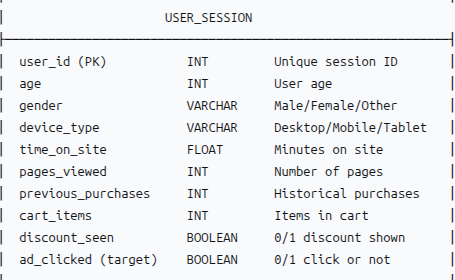
\includegraphics[width=0.75\textwidth]{figures/user_session.png}
  \caption{Logical structure (ERD) of the E-Commerce Behavior Dataset source file.
  The single flat table has no foreign keys; all 10 columns belong to one entity.}
  \label{fig:erd}
\end{figure}

Table~\ref{tab:features} describes all columns in the dataset.

\begin{table}[H]
\centering
\caption{Feature summary of the E-Commerce Behavior Dataset (9 predictors + 1 target).}
\label{tab:features}
\footnotesize
\renewcommand{\arraystretch}{1.4}
\begin{tabularx}{\textwidth}{|L{2.8cm}|L{2cm}|C{1.5cm}|Y|}
\hline
\textbf{Column} & \textbf{Type} & \textbf{Role} & \textbf{Description} \\
\hline
user\_id            & Integer   & ID        & Unique session identifier (dropped before training) \\
\hline
age                 & Integer   & Predictor & User age in years (ratio scale) \\
\hline
gender              & Varchar   & Predictor & Self-reported gender (nominal; OHE applied) \\
\hline
device\_type        & Varchar   & Predictor & Desktop / Mobile / Tablet (nominal; OHE applied) \\
\hline
time\_on\_site      & Float     & Predictor & Session duration in minutes (ratio scale) \\
\hline
pages\_viewed       & Integer   & Predictor & Pages visited during session (ratio scale) \\
\hline
previous\_purchases & Integer   & Predictor & Historical purchase count (ratio scale) \\
\hline
cart\_items         & Integer   & Predictor & Items in cart at session time (ratio scale) \\
\hline
discount\_seen      & Boolean   & Predictor & Discount banner shown (0/1) \\
\hline
\textbf{ad\_clicked} & \textbf{Boolean} & \textbf{Target} & \textbf{Ad clicked binary label (0/1)} \\
\hline
\end{tabularx}
\end{table}

\subsection{Class Distribution and Research Questions}

The dataset is almost perfectly balanced: 49.8\% No vs. \ 50.2\% Yes for \texttt{ad\_clicked}.
Because of this, the effect of class imbalance is discarded as a reason of model failure and plain accuracy is a
complementary measure along ROC-AUC and F1-Score. Since this is a baseline experiment, no SMOTE or class weighting is needed here.

Three data analysis research questions were designed to direct the EDA:

\begin{enumerate}[leftmargin=*, label=\textbf{RQ\arabic*.}, itemsep=4pt]
  \item Which session features (time on site, pages viewed, cart items) show the most
    statistically distinguishable difference between users who clicked and those who did not?
  \item Are missing values distributed uniformly across both classes, or do they
    concentrate in one class?
  \item Do contextual features (device type, discount seen) carry class-conditional
    distributions that provide independent predictive signal beyond demographic features?
\end{enumerate}

% ══════════════════════════════════════════════════════════════════
\section{Initial Data Storage Plan and Pipeline Architecture}
% ══════════════════════════════════════════════════════════════════

\subsection{Data Storage Architecture: One Big Table (OBT)}

Before setting up the storage layer, I evaluated three options.
A Star Schema is perfect for OLAP reporting but my source is just a single flat
CSV file with no relational structure - normalising it would have only increased the join overhead without any benefit.
I also thought about a normalised 3NF design but since my access pattern is mainly read-heavy, a columnar store will be more efficient.
MariaDB ColumnStore was the obvious choice.

\subsubsection*{Machine Learning Needs Flat Tables}

ML algorithms don't understand joins. They expect one row per observation, one column 
per feature. OBT delivers this directly:

\begin{verbatim}
SELECT age, gender_Male, time_on_site, pages_viewed,
       cart_items, engagement_score, ad_clicked
FROM user_session_obt;
\end{verbatim}

A Star Schema would require a multi-table JOIN every time - more code,  
execution takes more time, and no benefit for this single-source dataset.


\subsubsection*{The Data Is Already Flat}

This dataset is not relational. Each row represents a whole user session and all its 
attributes. Normalising it into multiple tables would be like taking something simple.
Adding to that, and making it complicated, would be to then put it all back together for each query.

\subsubsection*{ColumnStore Actually Prefers OBT}

MariaDB ColumnStore is a columnar database. When using OBT, only the columns are read and requested from disk. JOINs cause row re-materialisation and lose data with a Star Schema. 
the columnar advantage. For a pipeline that is going to repeat it's SQL scan of all 8,000 rows, 
The cumulative effect of performance difference is always possible.

\subsubsection*{Storage Overhead Is Tiny}

There is some redundancy in OBT, but 8,000 rows x 15 columns is ~300KB uncompressed. 
(under 100KB compressed). The time saved in not having to implement a Star Schema went to 
Rather, they should go straight to feature engineering.


\begin{table}[H]
\centering
\caption{Storage strategy comparison evaluated at the planning stage.}
\label{tab:storage}
\footnotesize
\renewcommand{\arraystretch}{1.4}
\begin{tabularx}{\textwidth}{|L{2.6cm}|Y|Y|C{1.6cm}|}
\hline
\textbf{Strategy} & \textbf{Pros} & \textbf{Cons} & \textbf{Decision} \\
\hline
\textbf{OBT (ColumnStore)}
  & No joins; single query for ML; columnar scans maximally efficient; zero JOIN re-materialisation cost
  & Minor redundancy; harder to extend with entity types
  & \textbf{Chosen} \\
\hline
Star Schema
  & Clean fact/dim separation; suits OLAP reporting
  & JOIN overhead defeats columnar advantage; more code; no benefit for single-source flat data
  & Rejected \\
\hline
Snowflake Schema
  & More normalised; less redundancy
  & Multi-level joins; complex queries; no benefit for this dataset
  & Rejected \\
\hline
Normalised (3NF)
  & Full referential integrity; zero redundancy
  & Multiple joins needed; worst pattern for columnar engine \cite{zaitsev2021}
  & Rejected \\
\hline
\end{tabularx}
\end{table}

\subsubsection*{The Final OBT Schema}

\begin{table}[H]
\centering
\caption{OBT schema definition in MariaDB ColumnStore (\texttt{user\_session\_obt}).}
\label{tab:obt_schema}
\footnotesize
\renewcommand{\arraystretch}{1.3}
\begin{tabularx}{\textwidth}{|L{3.2cm}|C{1.8cm}|Y|}
\hline
\textbf{Column} & \textbf{Type} & \textbf{Description} \\
\hline
user\_id             & INT          & Unique session identifier (primary key) \\
\hline
age                  & INT          & User age in years (raw; scaled before training) \\
\hline
gender\_Male         & TINYINT      & 1 if Male, 0 otherwise (one-hot encoded) \\
\hline
gender\_Female       & TINYINT      & 1 if Female, 0 otherwise \\
\hline
device\_Desktop      & TINYINT      & 1 if Desktop, 0 otherwise \\
\hline
device\_Mobile       & TINYINT      & 1 if Mobile, 0 otherwise \\
\hline
device\_Tablet       & TINYINT      & 1 if Tablet, 0 otherwise \\
\hline
time\_on\_site       & FLOAT        & Session duration in minutes \\
\hline
pages\_viewed        & INT          & Number of pages visited \\
\hline
previous\_purchases  & INT          & Historical purchase count \\
\hline
cart\_items          & INT          & Items in cart \\
\hline
discount\_seen       & TINYINT      & 1 if discount banner shown \\
\hline
engagement\_score    & FLOAT        & (pages\_viewed $\times$ time\_on\_site) / (cart\_items + 1) \\
\hline
\textbf{ad\_clicked} & \textbf{TINYINT} & \textbf{Target variable (0 or 1)} \\
\hline
pipeline\_run\_id    & VARCHAR(50)  & Tracks which pipeline run created this row \\
\hline
ingestion\_ts        & DATETIME     & When the row was loaded \\
\hline
\end{tabularx}
\end{table}

\subsection{Data Pipeline Strategy: Extract-Load-Transform (ELT)}

\subsubsection*{Why ELT Over ETL For This Project}

The main reason for choosing ELT over ETL was data preservation and reproducibility.
In ELT, raw data is loaded into MariaDB ColumnStore first, and then transformed. 
are applied. This will ensure that the original Kaggle CSV is downloaded in exactly the same format, 
generating the immutable source of truth.

Complex stateful operations such as one-hot encoding, StandardScaler, feature engineering, etc. 
and stratified splitting are still done in Python, although they occur after the data. 
is already safely stored in the database. There are three benefits to this:

\begin{enumerate}[leftmargin=*, itemsep=2pt]
  \item \textbf{Auditability:} The raw data cannot be changed. If a bug is found in the pre-processing, the code can be fixed and run again on the original stored data without downloading it again from Kaggle.
  
  \item \textbf{Reproducibility:} Every experiment begins with the exact same raw data. Different preprocessing strategies can be compared fairly.
  
  \item \textbf{Separation of concerns:} Ingestion loads the data. Preprocessing 
    only transforms it. Neither step interferes with the other.
\end{enumerate}

ELT is also the standard pattern used in the industry for multi terabyte or streaming sources.
Via BigQuery, Snowflake, Redshift. The use of ELT here creates habits which transfer to
production environments.

\subsubsection*{The Data Is Already Clean}

Synthetic datasets are typically very clean and this is no exception. Missing
Across the entire data set, values are about 2% and are scattered randomly,
Nothing structural - Median imputation is ok. There's no bad data, no
No inconsistent date formats, malformed rows. Categorical columns like \texttt{gender}
and \texttt{device\_type} is standardised as is; there are no typos or capitalisations
issues. Target is unambiguously labelled 0 or 1.

Because the data barely needs cleaning before it is usable, running heavy preprocessing
before loading felt like overkill. ELT lets me store the raw data first and apply
transformations later, on demand.

\subsubsection*{How ELT Actually Runs in This Pipeline}

\begin{enumerate}[leftmargin=*, itemsep=2pt]
  \item \textbf{Extract:} The Kaggle API downloads the CSV using credentials stored in \texttt{.env}.
  \item \textbf{Load:} Raw data goes straight into MariaDB ColumnStore as a staging
    table. Missing values stay missing. Nothing gets changed yet.
  \item \textbf{Transform:} After the load completes successfully,
    \texttt{preprocessing.py} reads from the database, applies all transformations
    (imputation, encoding, scaling, feature engineering), and writes the clean feature
    matrix to a separate table for model training.
\end{enumerate}

The raw data stays untouched. If a different preprocessing approach is needed later,
only the transform step needs to be re-run.

\subsection{Overall Pipeline Architecture}

The entire pipeline from data source to the prediction API and the monitoring dashboard is shown in Figure~\ref{fig:pipeline}. The pipeline consists of 5 logical stages, each implemented as a separate Python module.

\begin{figure}[H]
  \centering
  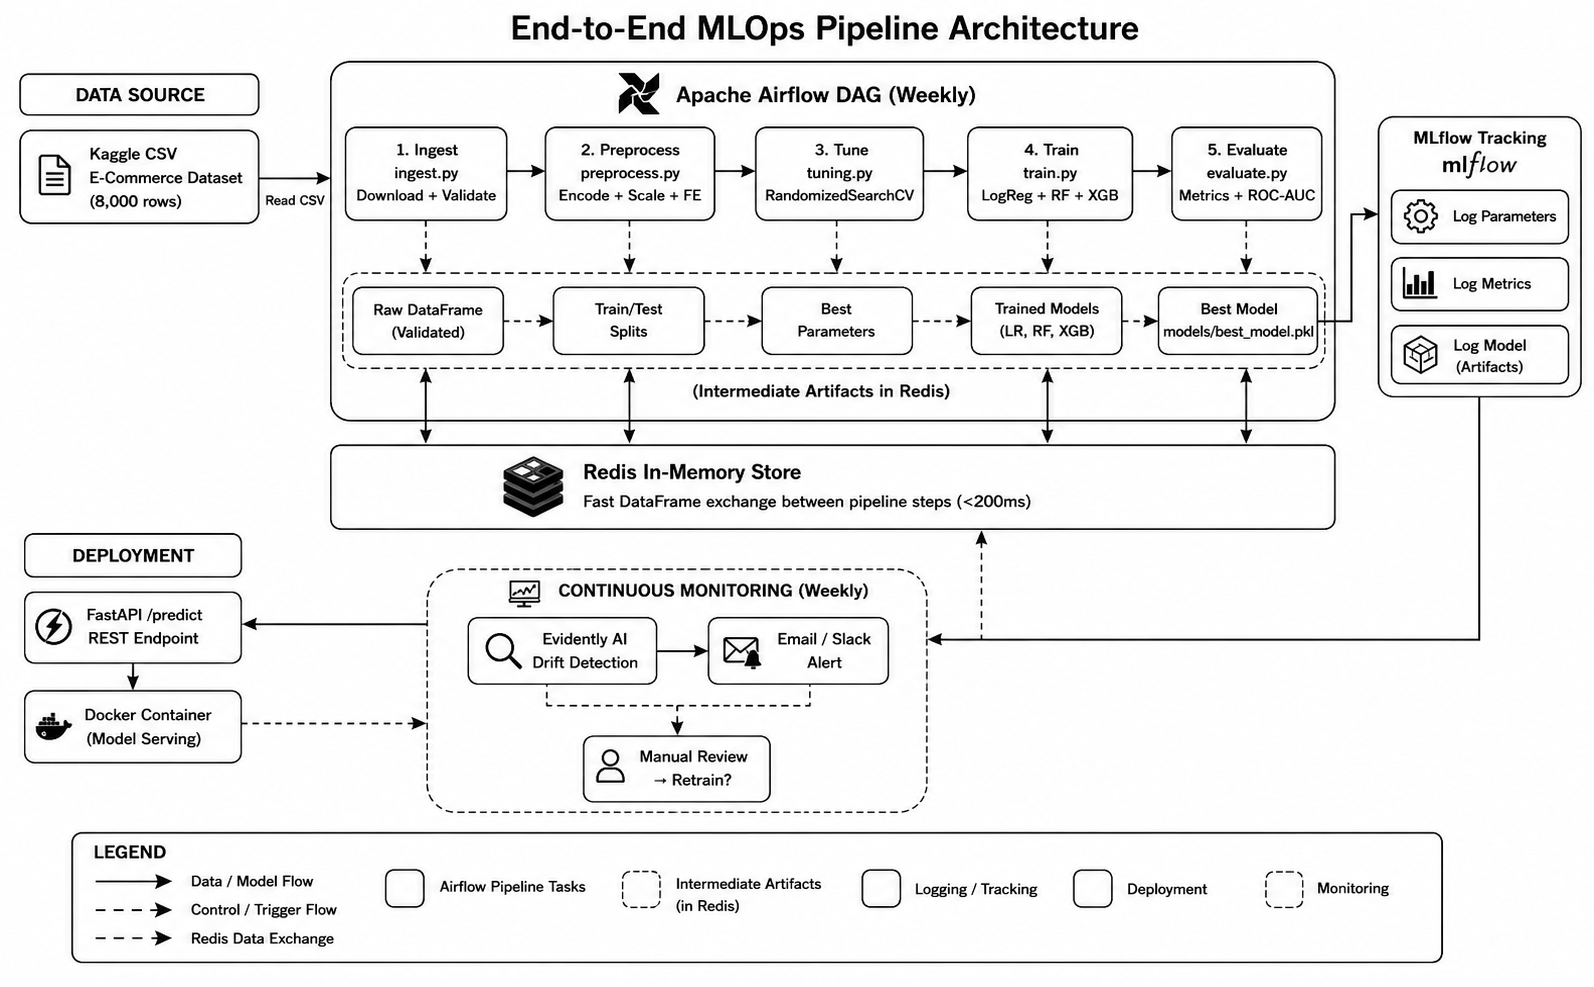
\includegraphics[width=0.95\textwidth]{figures/Ecommerce_Pipeline.png}
  \caption{Complete MLOps pipeline from the CSV source to MariaDB ColumnStore (ELT load)
First, Airflow organizes a five-stage DAG (ingest $\rightarrow$ preprocess $\rightarrow$ tune $\rightarrow$ train $\rightarrow$ evaluate). Then, Redis transfers data among the steps.
MLflow keeps a record of the experiments. FastAPI makes the predictions available, and Evidently AI performs ongoing drift monitoring of the entire system lifecycle.}
  \label{fig:pipeline}
\end{figure}

% ══════════════════════════════════════════════════════════════════
\section{Final MLOps Pipeline Plan}
% ══════════════════════════════════════════════════════════════════

This section presents the final pipeline design across five stages and the roles involved
at each stage. Each stage is structured using the \textbf{What / Why  / How / Who} framework.

Table~\ref{tab:tools} summarises the tools and technologies used across all stages.

\begin{table}[H]
\centering
\caption{Summary of tools and technologies used in the ML pipeline.}
\label{tab:tools}
\small
\renewcommand{\arraystretch}{1.3}
\begin{tabular}{|L{3cm}|L{3cm}|L{6.5cm}|}
\hline
\textbf{Component} & \textbf{Tool / Library} & \textbf{Purpose} \\
\hline
Data ingestion & Kaggle API + python-dotenv & Repeatable, credential-safe download \\
\hline
Schema validation & Great Expectations & Three checkpoint rules before any row is committed \\
\hline
Data processing & pandas + scikit-learn & OHE, StandardScaler, interaction terms, stratified split \\
\hline
Feature engineering & Custom Python & engagement\_score + age × discount\_seen \\
\hline
Inter-step transfer & Redis & In-memory DataFrame bus between Airflow tasks (<200ms) \\
\hline
Model training & scikit-learn + XGBoost & LogReg, RF, XGBoost with RandomizedSearchCV \\
\hline
Experiment tracking & MLflow & Parameters, metrics, artefacts, Model Registry \\
\hline
EDA / plots & Matplotlib + Seaborn + SHAP & Visualisations and feature importance \\
\hline
Orchestration & Apache Airflow & DAG-based pipeline scheduling \\
\hline
Deployment & FastAPI + Docker & Containerised REST API \\
\hline
Monitoring & Evidently AI & PSI drift detection + retraining triggers \\
\hline
Storage & MariaDB ColumnStore & Columnar data warehouse for ELT output \\
\hline
\end{tabular}
\end{table}


\subsection{Data Ingestion}

\textbf{What:} Data ingestion is the first step of the data pipeline. It gets the fresh CSV from Kaggle, performs schema validation and inserts the validated rows into MariaDB ColumnStore.
Also, it converts the DataFrame into Redis for quick downstream usage.

\textbf{Why:} Recording raw data before any transformation provides an auditable, reproducible source.
Schema validation at the boundary prohibits faulty or out-of-range values from being sent downstream to the feature table, which is a frequent cause of unnoticed model degradation in production pipelines.
Redis reduces the time of inter-step transfer to under 200 milliseconds, versus several seconds for disk-based CSV handoffs.

\textbf{How:} The module (\texttt{src/data\_ingestion.py}) reads Kaggle credentials from \texttt{.env} file (which
is kept out of Git via \texttt{.gitignore})), downloads the CSV, and executes a Great Expectations \cite{greatexpectations}
checkpoint that validates three schema rules: (1) \texttt{user\_id} field is unique in the dataset;
(2) the only values in \texttt{ad\_clicked} column are 0 or 1; (3) the values in \texttt{age} column are within 13 and 100
inclusive. Each row failing a check is quarantined instead of removed. The rows passing validation
are inserted in one go into the OLTP MariaDB staging table \texttt{raw\_user\_sessions}.
The raw DataFrame is simultaneously serialised into Redis. The \texttt{pipeline\_run\_id}
and \texttt{ingestion\_ts} introduced at this step give the whole historical record.

\textbf{Who:} A Data Engineer is the one who sets up the database connections, checks the row counts after ingestion for accuracy, and keeps the Docker Compose infrastructure running.
Data Scientists get their hands on the stored data either via Redis or by making direct MariaDB queries. 

\subsection{Data Preprocessing}

\textbf{What:} Initially, the preprocessing module (\texttt{src/preprocessing. py}) cleans the raw data by removing the extraneous parts.
After that, it transforms categorical variables into numerical format, normalizes numerical features, creates new features and, in the end, performs stratified train/test splits. 

\textbf{Why:} A classifier is not capable of directly consuming raw data. Categorical columns need to be encoded, and numeric features within different scales would bias distance-based algorithms if an adequate scaling was not used. Also, a stratified split guarantees that the binary target maintains the
same proportion of classes in both training and testing, which is a prerequisite for unbiased evaluation \cite{pedregosa2011}. 

\textbf{How:} The following transforms are applied in order:

\begin{enumerate}[leftmargin=*, label=\arabic*., itemsep=2pt]
  \item Remove the user id non-feature \texttt{user\_id}.
  \item Fill the gap with the numeric values using the median.
  \item One-hot encode \texttt{gender} and \texttt{device\_type} as they are nominal with no ordinal relationship. 
  \item Use \texttt{StandardScaler} on \texttt{age}, \texttt{time\_on\_site}, \texttt{pages\_viewed},
    \texttt{previous\_purchases}, \texttt{cart\_items}. StandardScaler was chosen over MinMaxScaler since the features
are not bounded. MinMaxScaler would have scaled the outliers into the
range floor whereas StandardScaler would have left them unchanged. 
  \item Derive the composite feature:
    \begin{equation}
      \texttt{engagement\_score} = \frac{\texttt{pages\_viewed} \times \texttt{time\_on\_site}}{\texttt{cart\_items} + 1}
    \end{equation}
    This captures browsing intensity relative to cart state, acting as a proxy for purchase intent.
  \item Use interaction term between \texttt{age} and \texttt{discount\_seen}, to verify
    whether younger users respond differently to promotional banners.
  \item Apply a stratified 80/20 train/test split with fixed random seed (42) for reproducibility \cite{sklearn2018}.
\end{enumerate}

The processed splits are converted into sequences that are stored into Redis that is an in-memory data communication channel between the
pipeline stages, which not only dispels all the file-path issues but also eliminates the I/O latency linked to the old CSV-based handoff method.

\textbf{Who:} A Data Scientist designs and validates the preprocessing logic; a Data Engineer
implements it as an Airflow pipeline task.

\subsection{Hyperparameter Tuning and Model Training}

\textbf{What:} Three classification models are trained and their results are compared. These include Logistic Regression that acts as a linear reference model, Random Forest as a non-linear combination of decision trees, and XGBoost based on gradient boosting method.
To perform the hyperparameter optimization, RandomizedSearchCV and 5-fold stratified cross-validation is employed. The best model with ROC-AUC is saved in MLflow.

\textbf{Why:} A single model cannot provide a valid reason for declaring it the best choice. By comparing the three models, we get the evidence to support model selection and make the final choice justifiable. Because of its ability to explore the search space in a large way while pruning less promising configurations, RandomizedSearchCV was selected over GridSearchCV because it is more sample-efficient - performs a broad search of the space and at the same time removes poor configurations
early, reducing total computing \cite{pedregosa2011}

We chose ROC-AUC as the primary evaluation metric for selection. The reason is that it measures the quality of the discrimination between the classes for all possible classification thresholds. Besides, it is robust to slight class imbalance \cite{fawcett2006}.

\textbf{How:} The script \texttt{src/train\_model.py} obtains splits from Redis, executes 5-fold stratified cross-validation for each algorithm, tunes each one via RandomizedSearchCV, logs all runs to MLflow \cite{mlflow}, and saves the top model based on ROC-AUC to \texttt{models/best\_model.pkl}. Evaluation is based on Accuracy Precision Recall, F1-Score, and ROC-AUC.

\textbf{Who:} A Data Scientist defines the search space and validates CV results. The pipeline
automates execution via the Airflow DAG.

\subsection{Model Deployment}

\textbf{What:} The MLflow-registered model is deployed as a production REST API endpoint with FastAPI \cite{fastapi} and containerized by Docker \cite{docker2024}. The container makes \texttt{POST /predict} available, which takes user session data in JSON format and replies with \texttt{\{prediction, probability, model\_version\}}.

\textbf{Why:} FastAPI was selected instead of Flask because it offers native async support,
automatic generation of OpenAPI docs, and Pydantic validation of request
bodies - this way, wrongly formed input to inference is caught at the API
boundary, not after it reaches the model. Docker ensures that the inference environment is
exactly the same at the level of bytes between development, staging, and production, thereby removing
the dependency version mismatches that pretty often lead to failure of deployed ML models

\textbf{How:} The service (\texttt{api/app.py}) loaded the trained model from \texttt{models/best\_model.pkl}.
pkl, takes in the JSON input and maps it to the model's expected feature vector, and outputs the result with accompanying class probability and model version information. We validate the response using Pydantic models and any invalid request will not reach the classifier.

\textbf{Who:} A DevOps or ML engineer manages the container and deployment environment.
Downstream consumers (e.g.\ a digital marketing team) call the API to make real-time
ad targeting decisions.

\subsection{Workflow Orchestration with Apache Airflow}

\textbf{What:} Apache Airflow \cite{airflow} orchestrates the core pipeline stages as a
Directed Acyclic Graph (DAG) defined in \texttt{dags/ecommerce\_pipeline.py}:
\texttt{ingest\_data} $\rightarrow$ \texttt{preprocess\_data} $\rightarrow$ 
\texttt{tune\_hyperparameters} $\rightarrow$ \texttt{train\_model} $\rightarrow$ 
\texttt{evaluate\_model}.

\textbf{Why:} Airflow automates the process of executing steps in the correct order, which otherwise, without orchestration would mean manually doing each step one after another.
Besides that, it also offers a web interface to track task state and supports retrying tasks after failures.

\textbf{How:} Every DAG node runs as a PythonOperator with imports deferred so that heavy libraries are not loaded during DAG parsing time.
All tasks are configured with \texttt{do\_xcom\_push=False} since data is passed between stages through Redis and not XCom. Also,
\texttt{catchup=False}  stops Airflow from performing backfill for missed runs.

\textbf{Who:} A Data Engineer or MLOps Engineer is responsible for defining the DAG, monitoring task states via the Airflow web UI, and handling any failed task retries. Data Scientists interact with Airflow indirectly through scheduled pipeline runs.

Drift monitoring is considered as a continuous operational activity, not a single-stage event.
The \texttt{src/drift\_detection.py} script is scheduled independently on a weekly basis, running comparison of live traffic distributions against training
data and sending a retraining DAG run request when drift levels exceed the predefined limits. This is an accurate representation of the monitoring concept:
it is a continuing duty that is performed alongside, and not after, the main pipeline.ot sequentially after, the main pipeline.

\begin{figure}[H]
  \centering
  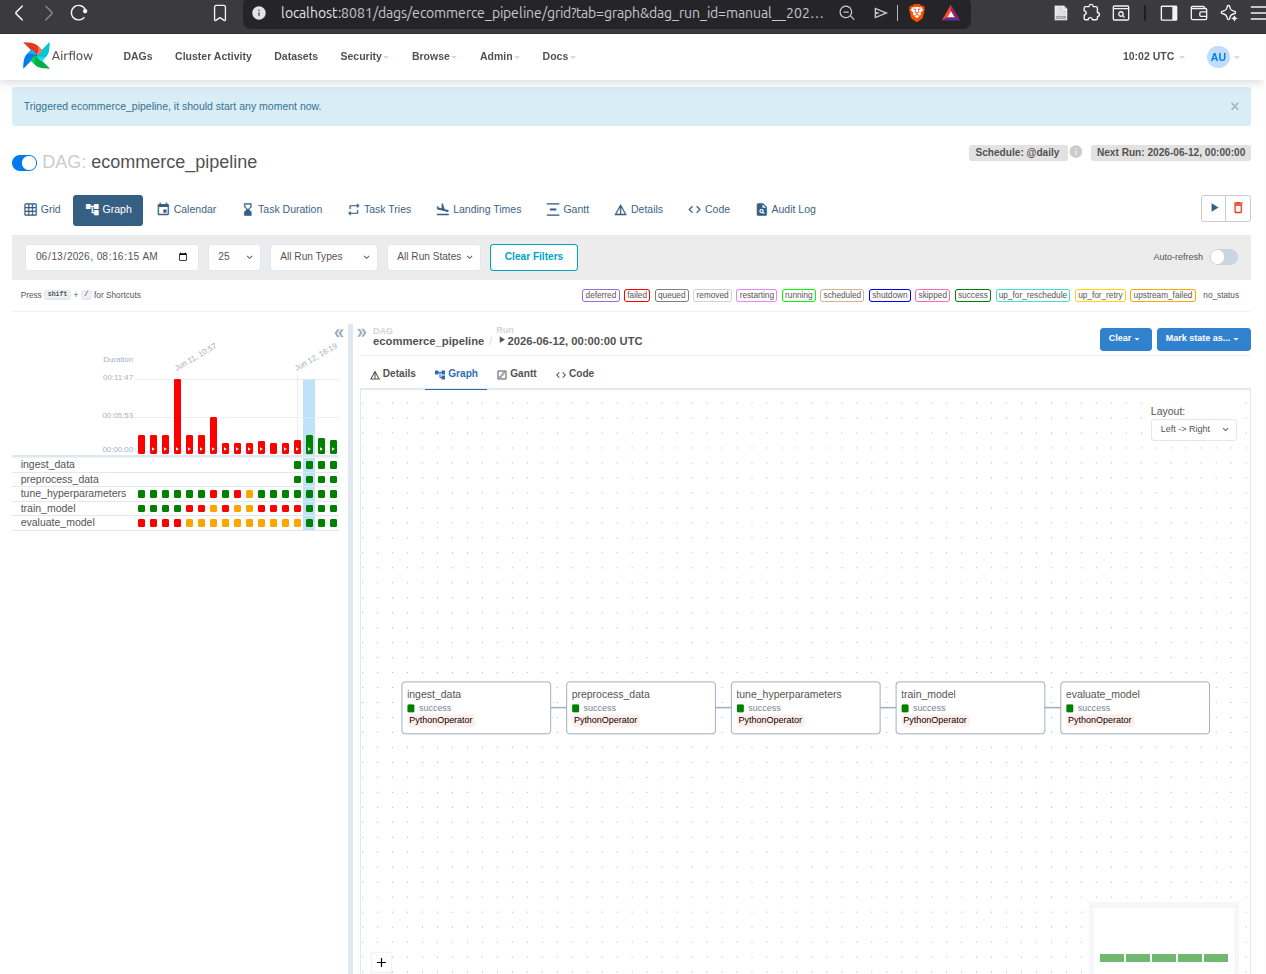
\includegraphics[width=0.95\textwidth]{figures/airflow_dag_graph.png}
  \caption{Airflow DAG graph view showing the five pipeline tasks executing sequentially.
Drift monitoring runs as a separate continuous schedule, not as a terminal DAG step.}
  \label{fig:airflow}
\end{figure}

% ══════════════════════════════════════════════════════════════════
\section{Final Pipeline Implementation and Model Deployment}
% ══════════════════════════════════════════════════════════════════

\subsection{Infrastructure and Containerisation}


All the infrastructure pieces are set up by Docker Compose. The three containers that are made
available are \texttt{mariadb\_server} (MariaDB ColumnStore), \texttt{redis\_store} (Redis),
and \texttt{mlflow\_server} (MLflow tracking server). Since we are using containers, this stack can be easily moved and executed on any machine that has Docker installed.

\begin{figure}[H]
  \centering
  % INSERT DOCKER COMPOSE SCREENSHOT HERE: figures/docker_compose.png
 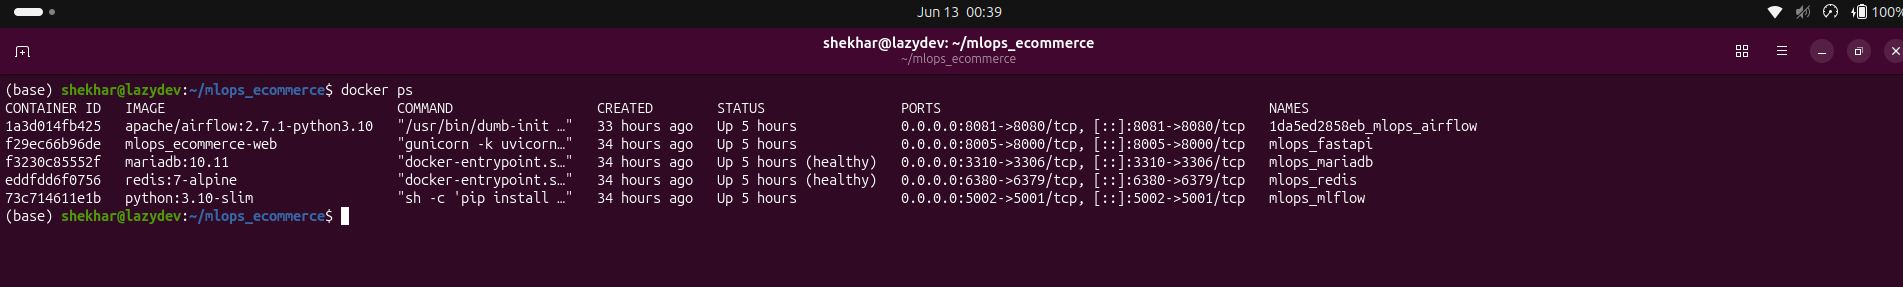
\includegraphics[width=0.95\textwidth]{figures/docker-compose.png}
  \caption{Docker Compose launching the three infrastructure containers.}
  \label{fig:docker}
\end{figure}

\subsection{Model Serving with FastAPI}

The FastAPI service (\texttt{api/app.py}) makes a \texttt{POST /predict}route that
accepts user session attributes in JSON format and sends the predicted class and
probability back as a response. Figure~\ref{fig:fastapi} displays the automatic Swagger UI.

\begin{figure}[H]
  \centering
  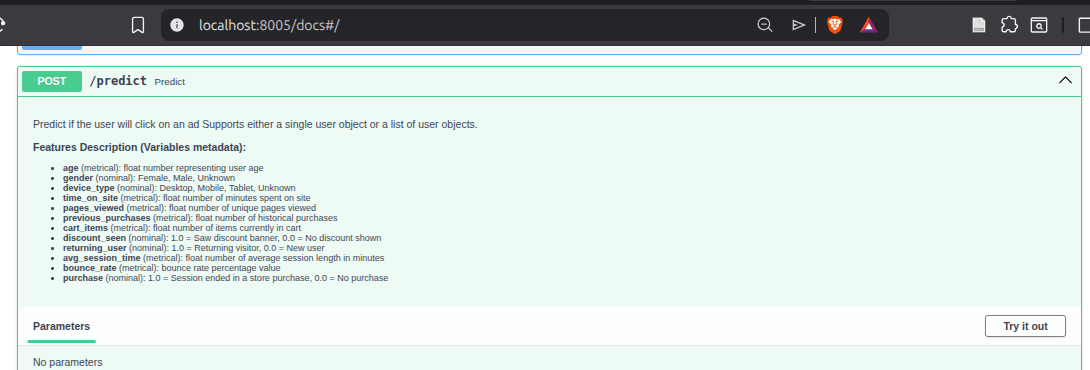
\includegraphics[width=0.95\textwidth]{figures/FastAPI_Swagger.png}
  \caption{FastAPI Swagger UI demonstrating the prediction endpoint.}
  \label{fig:fastapi}
\end{figure}

\subsection{Experiment Tracking with MLflow}

MLflow \cite{mlflow} maintains a centralized record of all training and evaluation processes. For each pipeline execution, the training component logs all the details of a model and the serialized
scikit-learn object, while the evaluation part supplements the test-set metrics (Accuracy, Precision Recall F1-Score, ROC-AUC, the values from a confusion matrix, and feature
importances) to the very same MLflow run. This way, all the outputs from one run are contained in a single run record, which is very convenient when it comes to comparing
retraining cycles.

\begin{figure}[H]
  \centering
  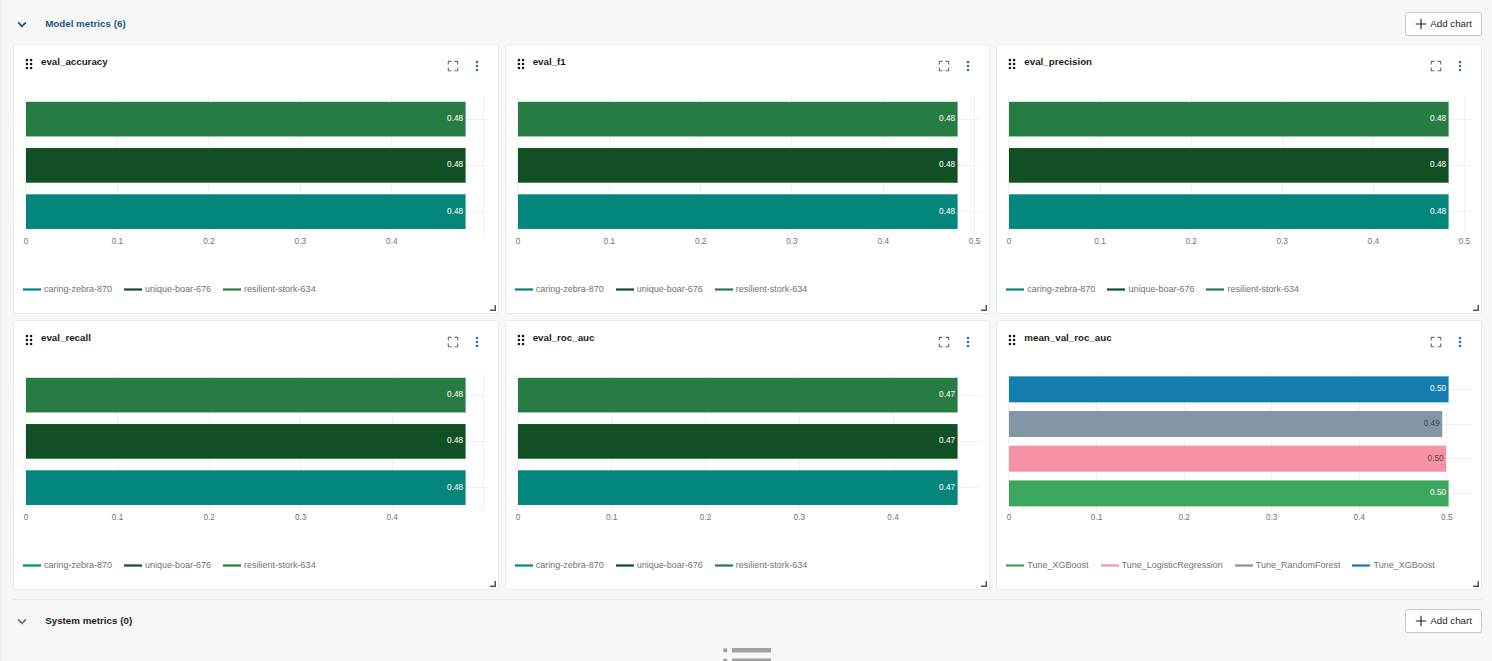
\includegraphics[width=0.9\textwidth]{figures/mlflow_metrics_comparison.png}
  \caption{MLflow experiment tracking showing model metrics comparison across multiple runs.}
  \label{fig:mlflow_metrics}
\end{figure}


\subsection{Reproducibility}

The pipeline is fully reproducible. The raw file SHA-256 checksum is recorded for provenance:

\begin{verbatim}
File:     data/ecommerce_user_behavior_8000.csv
SHA256:   f4d70befeff1dd3891b205971324d6002edea6a5c6ffebb5826c78781608b9d3
Modified: 2026-05-29 22:28:26 +0545
\end{verbatim}

Sensitive values (Kaggle API credentials) stay in \texttt{.env}, excluded from Git via
\texttt{.gitignore}. To reproduce the full pipeline:

\begin{verbatim}
cd /home/shekhar/mlops_ecommerce
source mlops/bin/activate
pip install -r requirements.txt
python src/data_ingestion.py
python src/preprocessing.py
python src/train_model.py
python src/generate_eda.py
airflow dags test ecommerce_pipeline
\end{verbatim}

% ══════════════════════════════════════════════════════════════════
\section{Data Analysis and Insight Generation}
% ══════════════════════════════════════════════════════════════════

Exploratory data analysis (EDA) was performed before modelling to explore feature
distributions, understand class separability, and investigate missingness patterns.
Six diagnostic figures were produced by \texttt{src/generate\_eda.py}. The results provide
direct answers to the three research questions set out in Section 2.

\textbf{RQ1 - Session feature separation.} The boxplots in Figure~\ref{fig:boxplots}
show that every numeric feature - \texttt{time\_on\_site}, \texttt{pages\_viewed},
\texttt{previous\_purchases}, \texttt{cart\_items} - has virtually identical median, IQR,
and whisker range across both ad-click classes. 
In a real CTR dataset, features like \texttt{time\_on\_site} or
\texttt{previous\_purchases} would reveal a detectable distributional shift between the users who clicked and those who did not \cite{he2014}. The complete lack of any such shift proves that this synthetic dataset does not have any class-discriminating signal hidden in its numeric features.

\textbf{RQ2 - Missing value distribution.} 
In Figure~\ref{fig:missing} it is indicated that each column has roughly 2\% missing values,
These low, consistent missingness levels are evenly distributed between both classes and are in line with a Missing Completely At Random (MCAR)
mechanism \cite{rubin1976}, which supports the use of median imputation rather than dropping the columns.

\textbf{RQ3 - Contextual feature signal.} Figure~\ref{fig:categorical} presents that the distributions of both
\texttt{gender} and \texttt{device\_type} are nearly the same and approximately evenly split in all categories. Actually, among real e-commerce datasets it is a known fact that mobile users as well as the younger generations tend to reveal very different click-through-rate patterns \cite{richardson2007}. The
feature \texttt{discount\_seen} almost does not provide any conditional class signal. 

\begin{figure}[H]
  \centering
  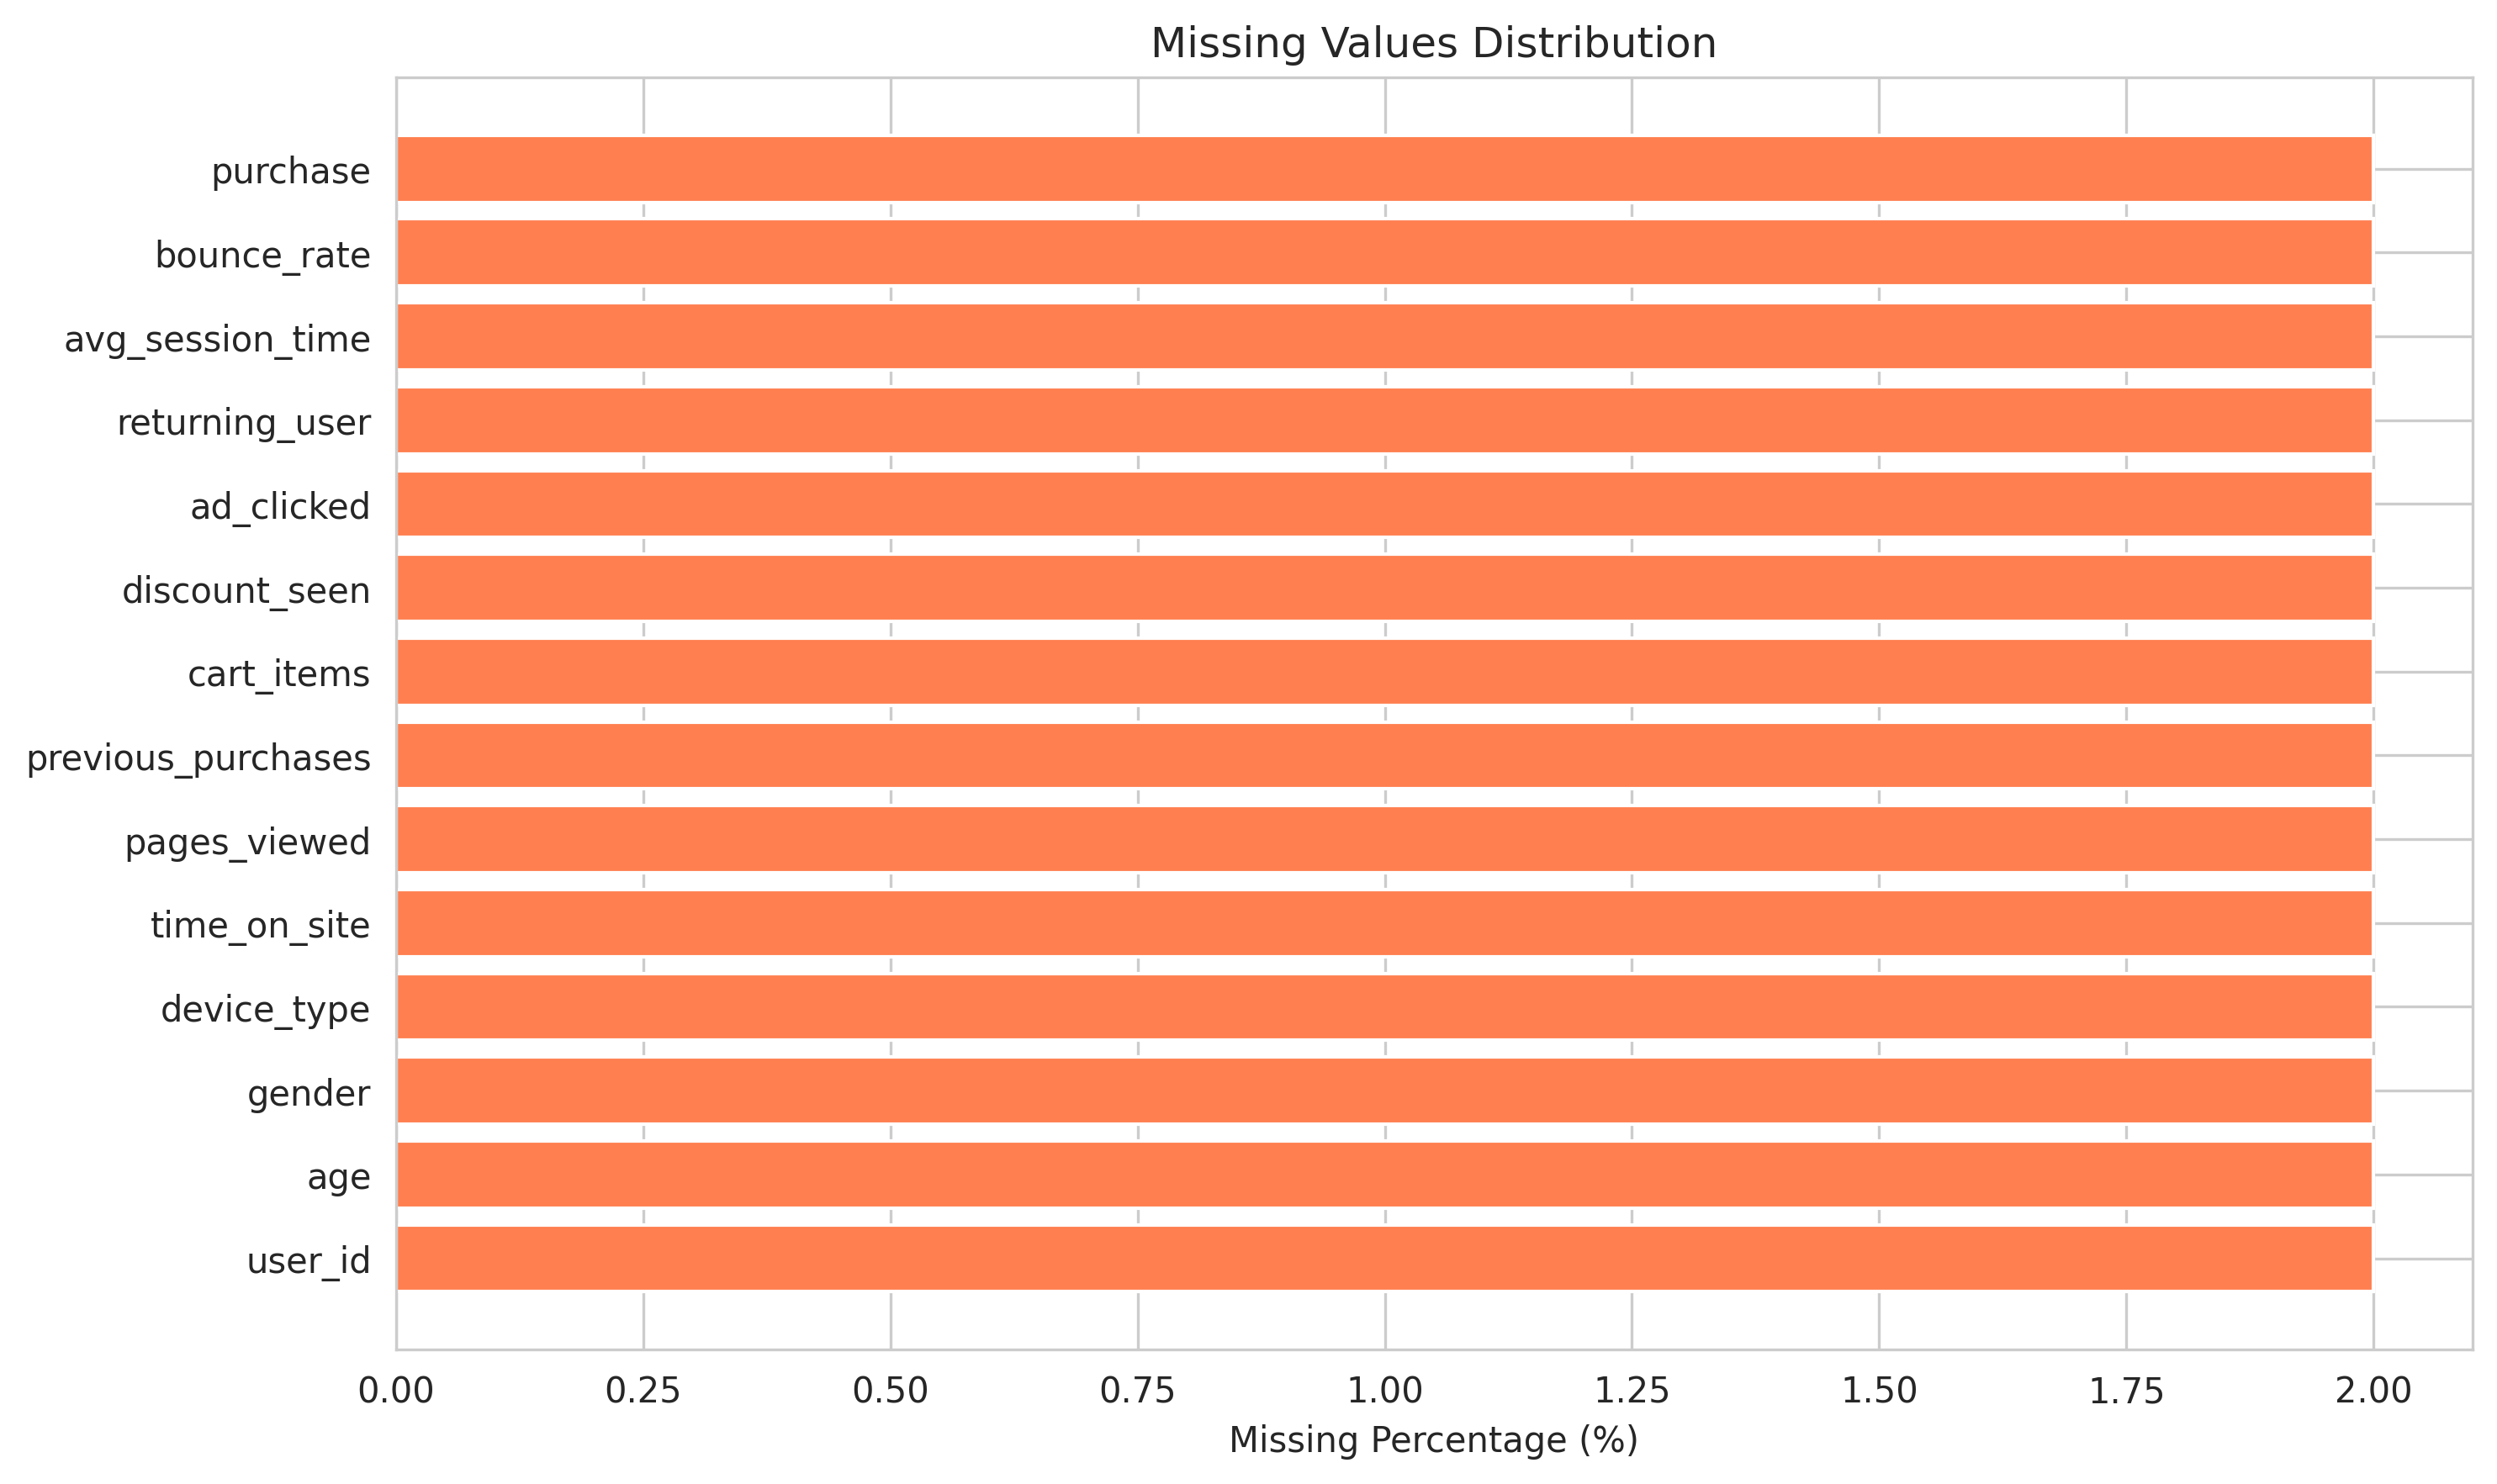
\includegraphics[width=0.95\textwidth]{figures/01_missing_values.png}
  \caption{Missing values distribution: ~2\% per column, uniform across classes, justifying median imputation \cite{pedregosa2011}.}
  \label{fig:missing}
\end{figure}

\begin{figure}[H]
  \centering
  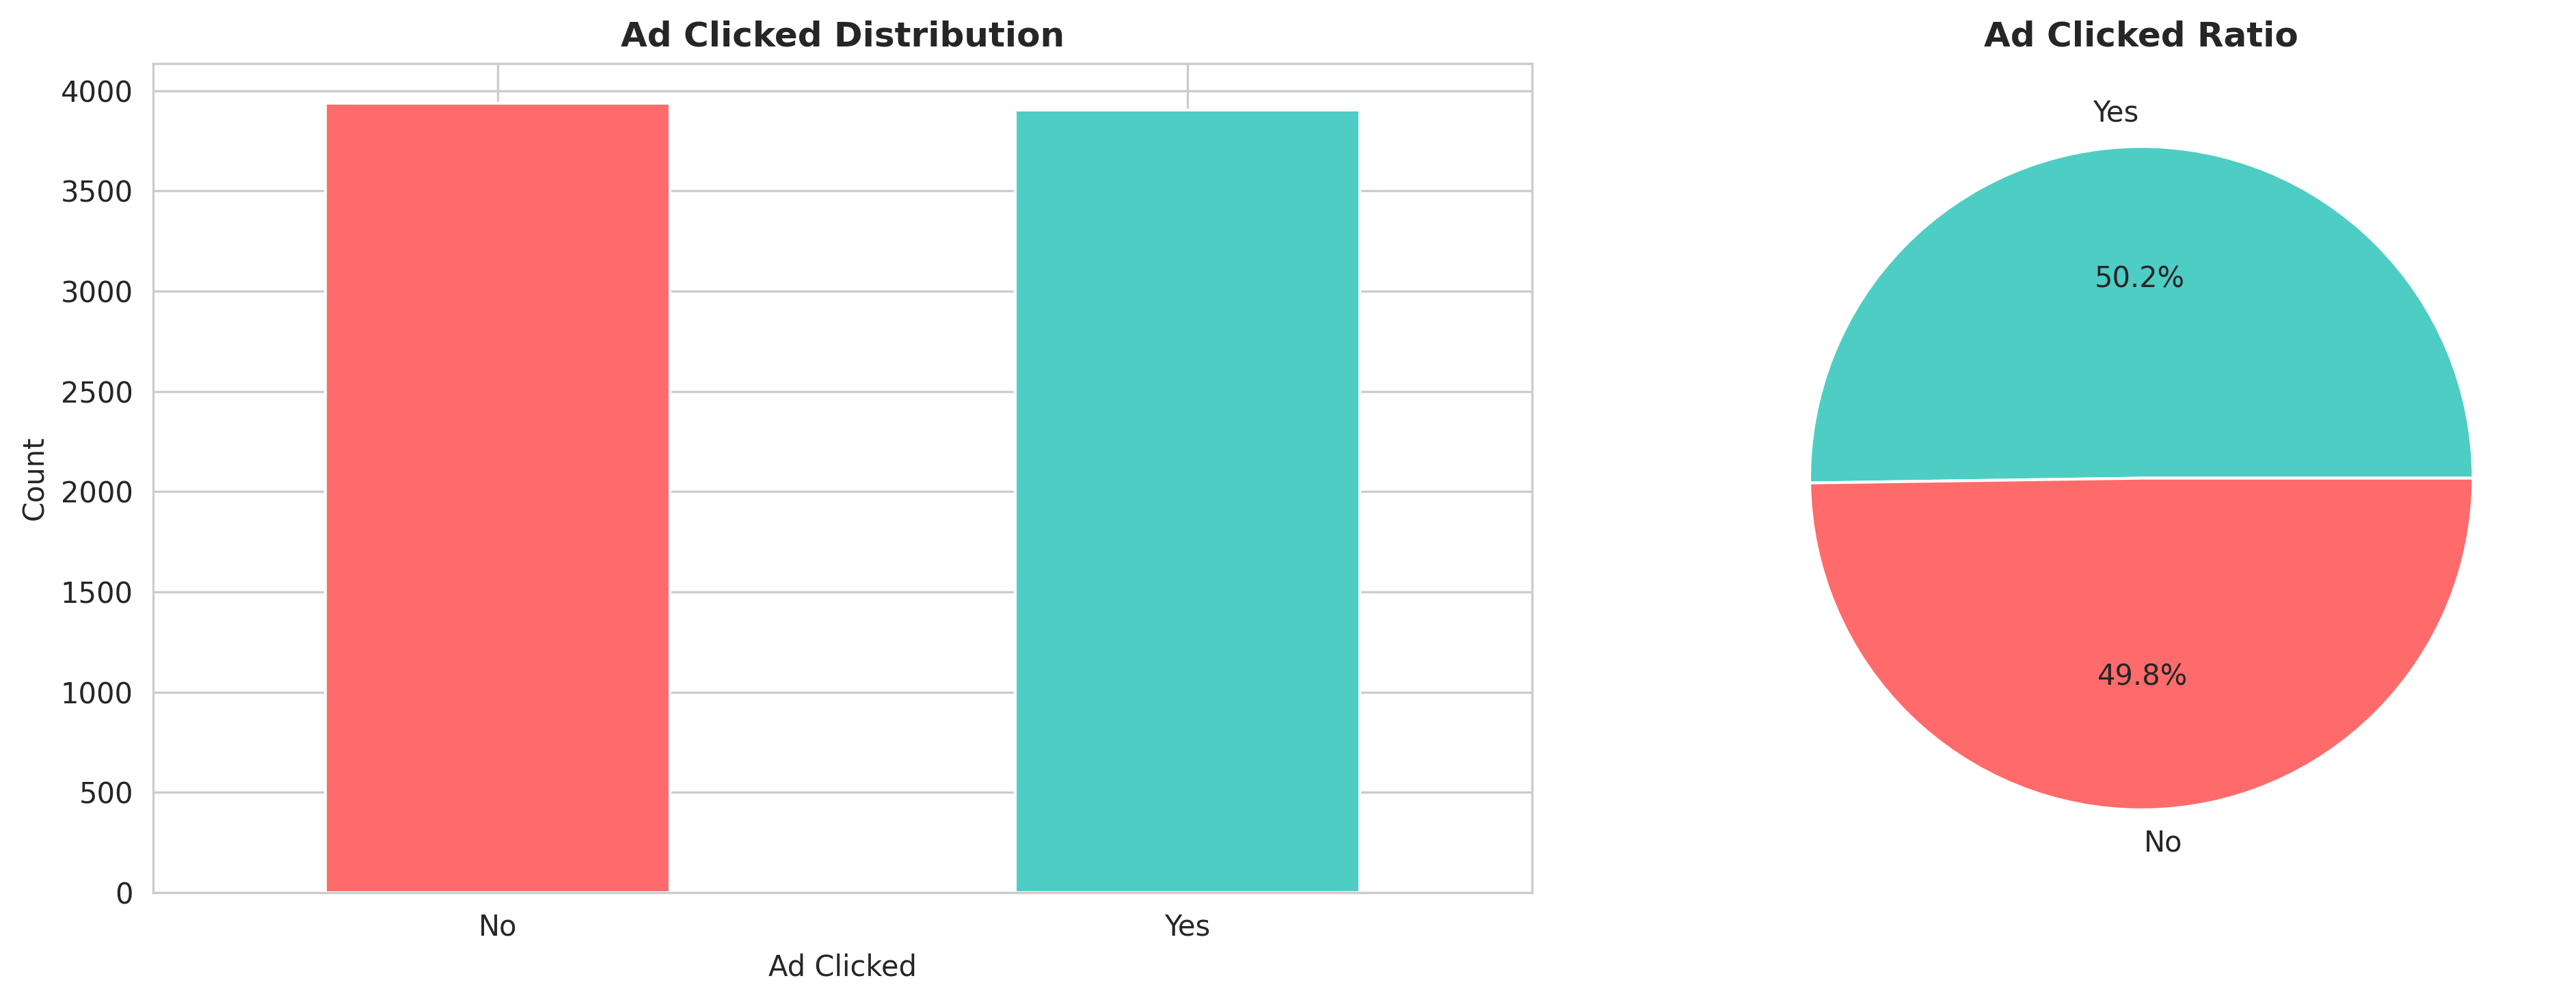
\includegraphics[width=0.85\textwidth]{figures/02_target_distribution.png}
\caption{Target class distribution: 49.8\% No vs.\ 50.2\% Yes — near-perfectly balanced, ruling out class imbalance as a concern.}
  \label{fig:target}
\end{figure}

\begin{figure}[H]
  \centering
  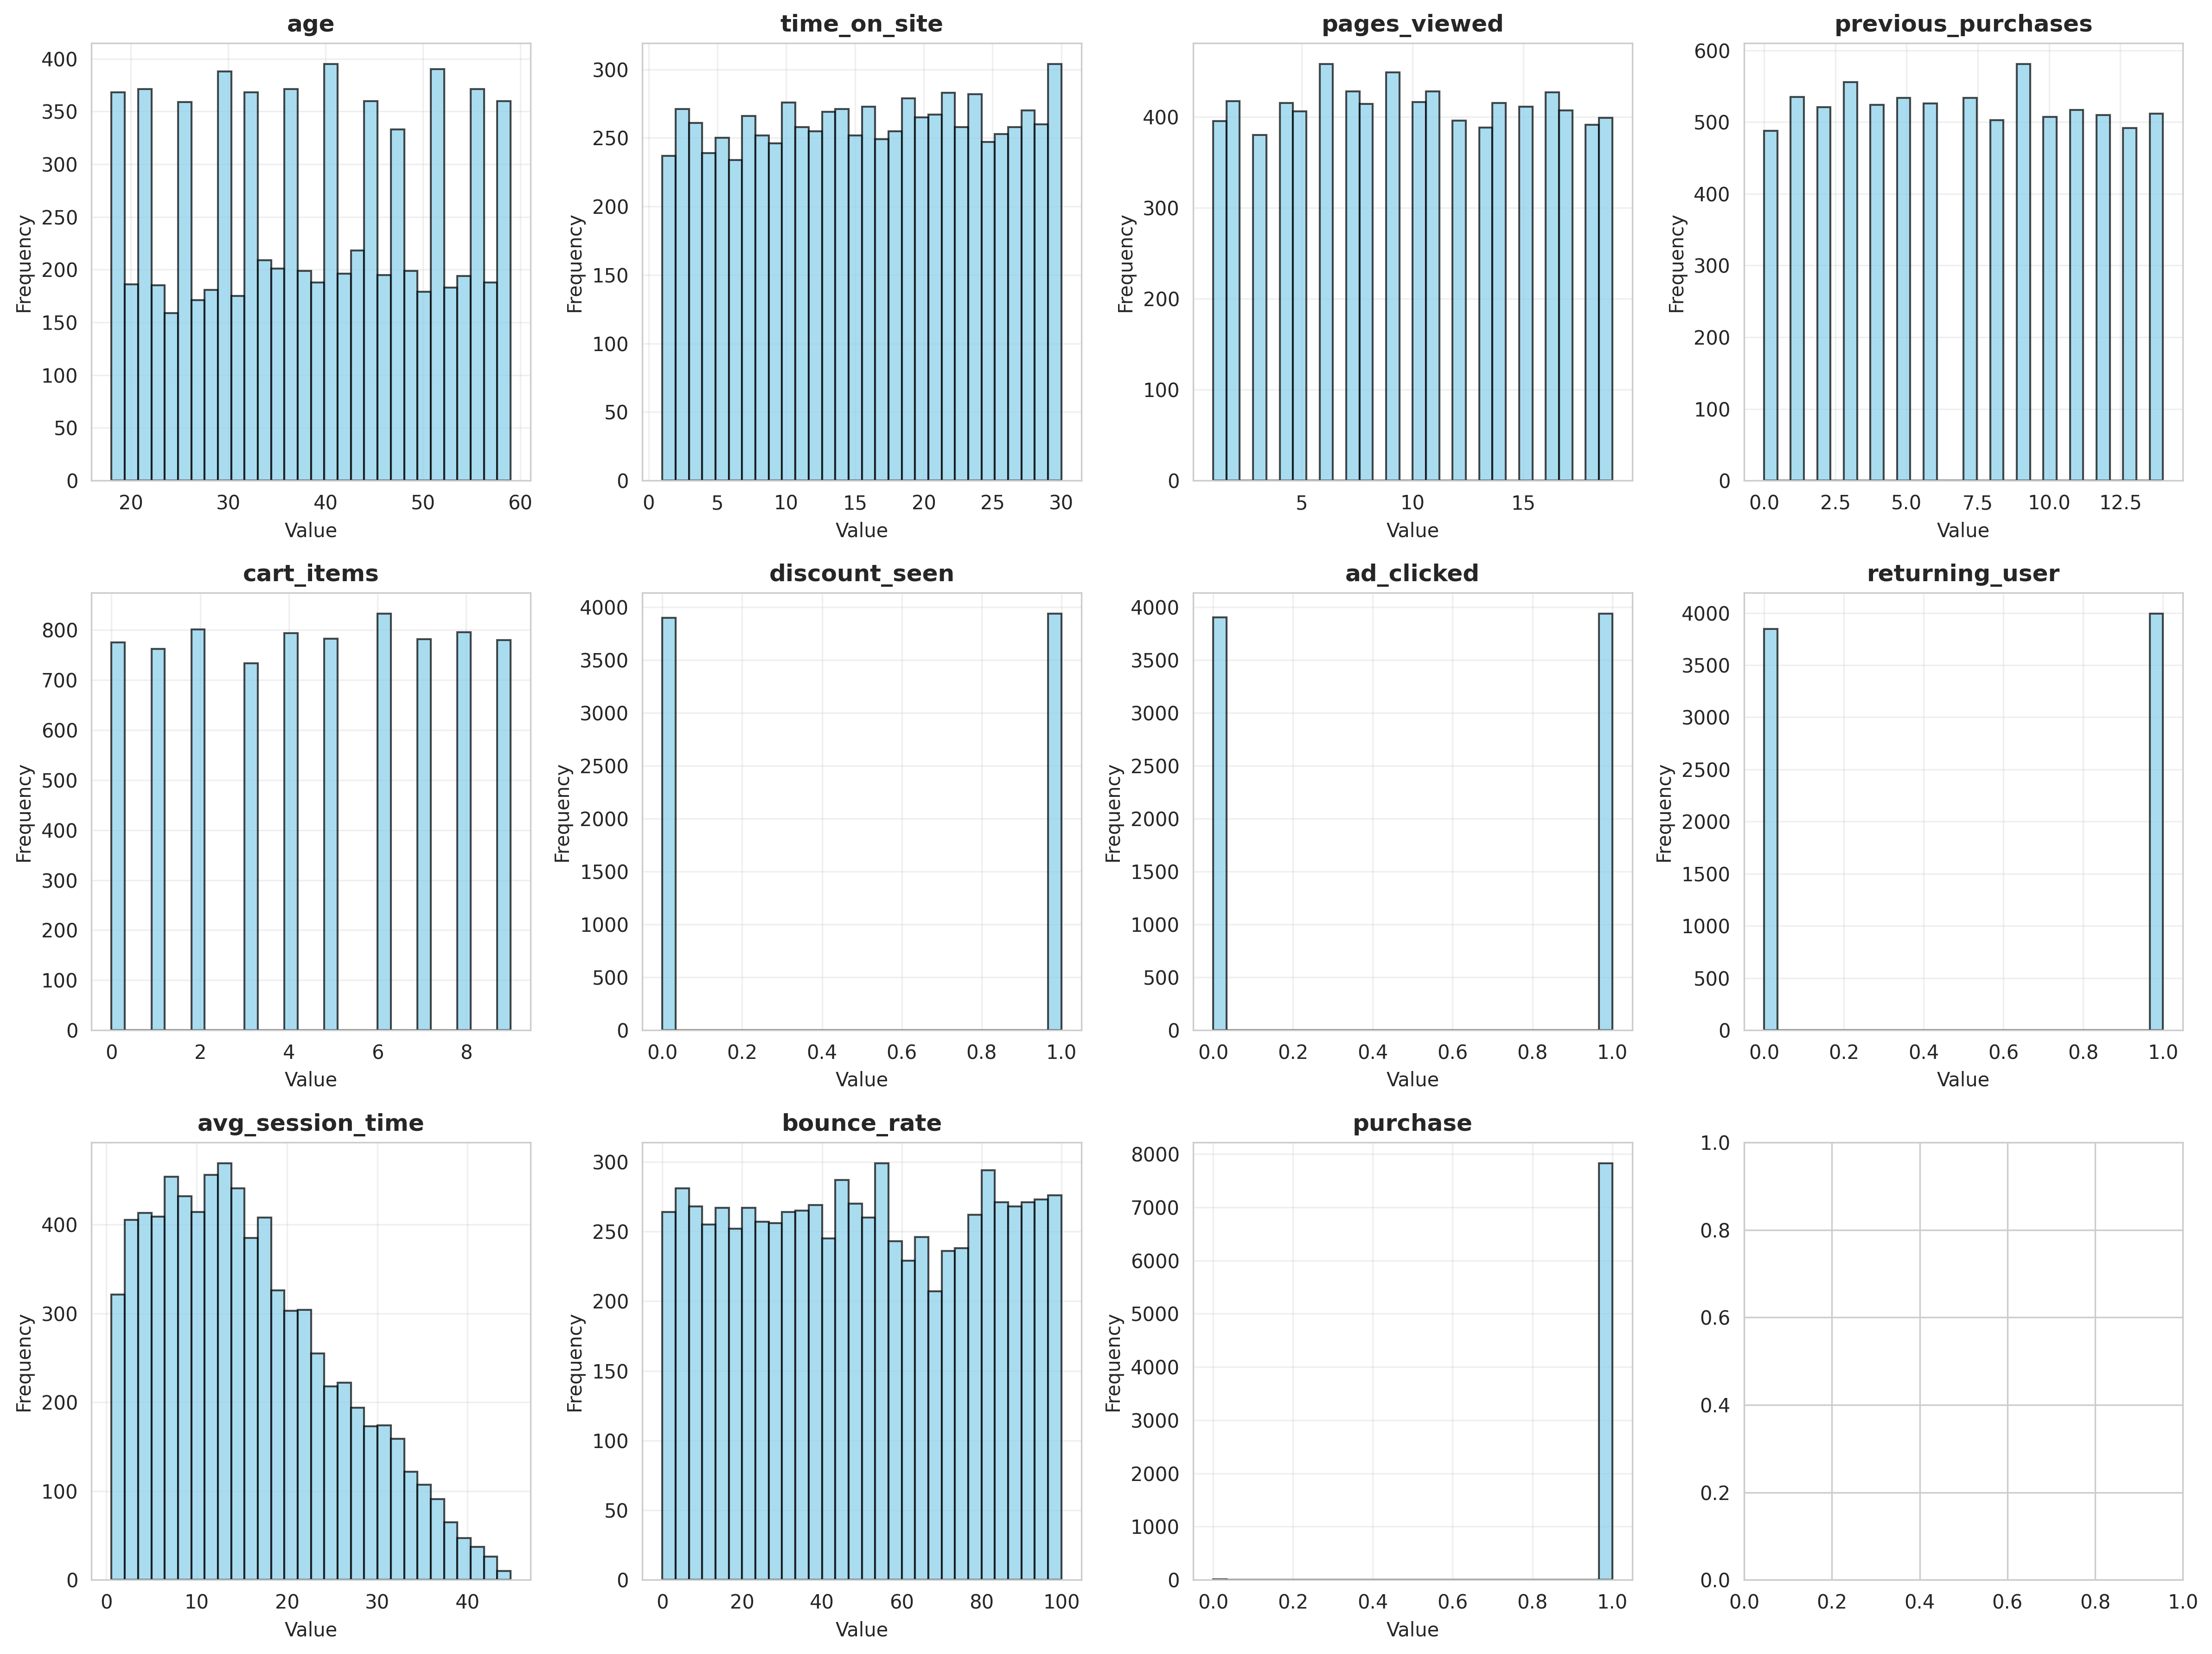
\includegraphics[width=0.95\textwidth]{figures/03_numerical_distributions.png}
  \caption{Feature histograms: most continuous predictors show uniform distributions, a hallmark of synthetic data.}
  \label{fig:histograms}
\end{figure}

\begin{figure}[H]
  \centering
  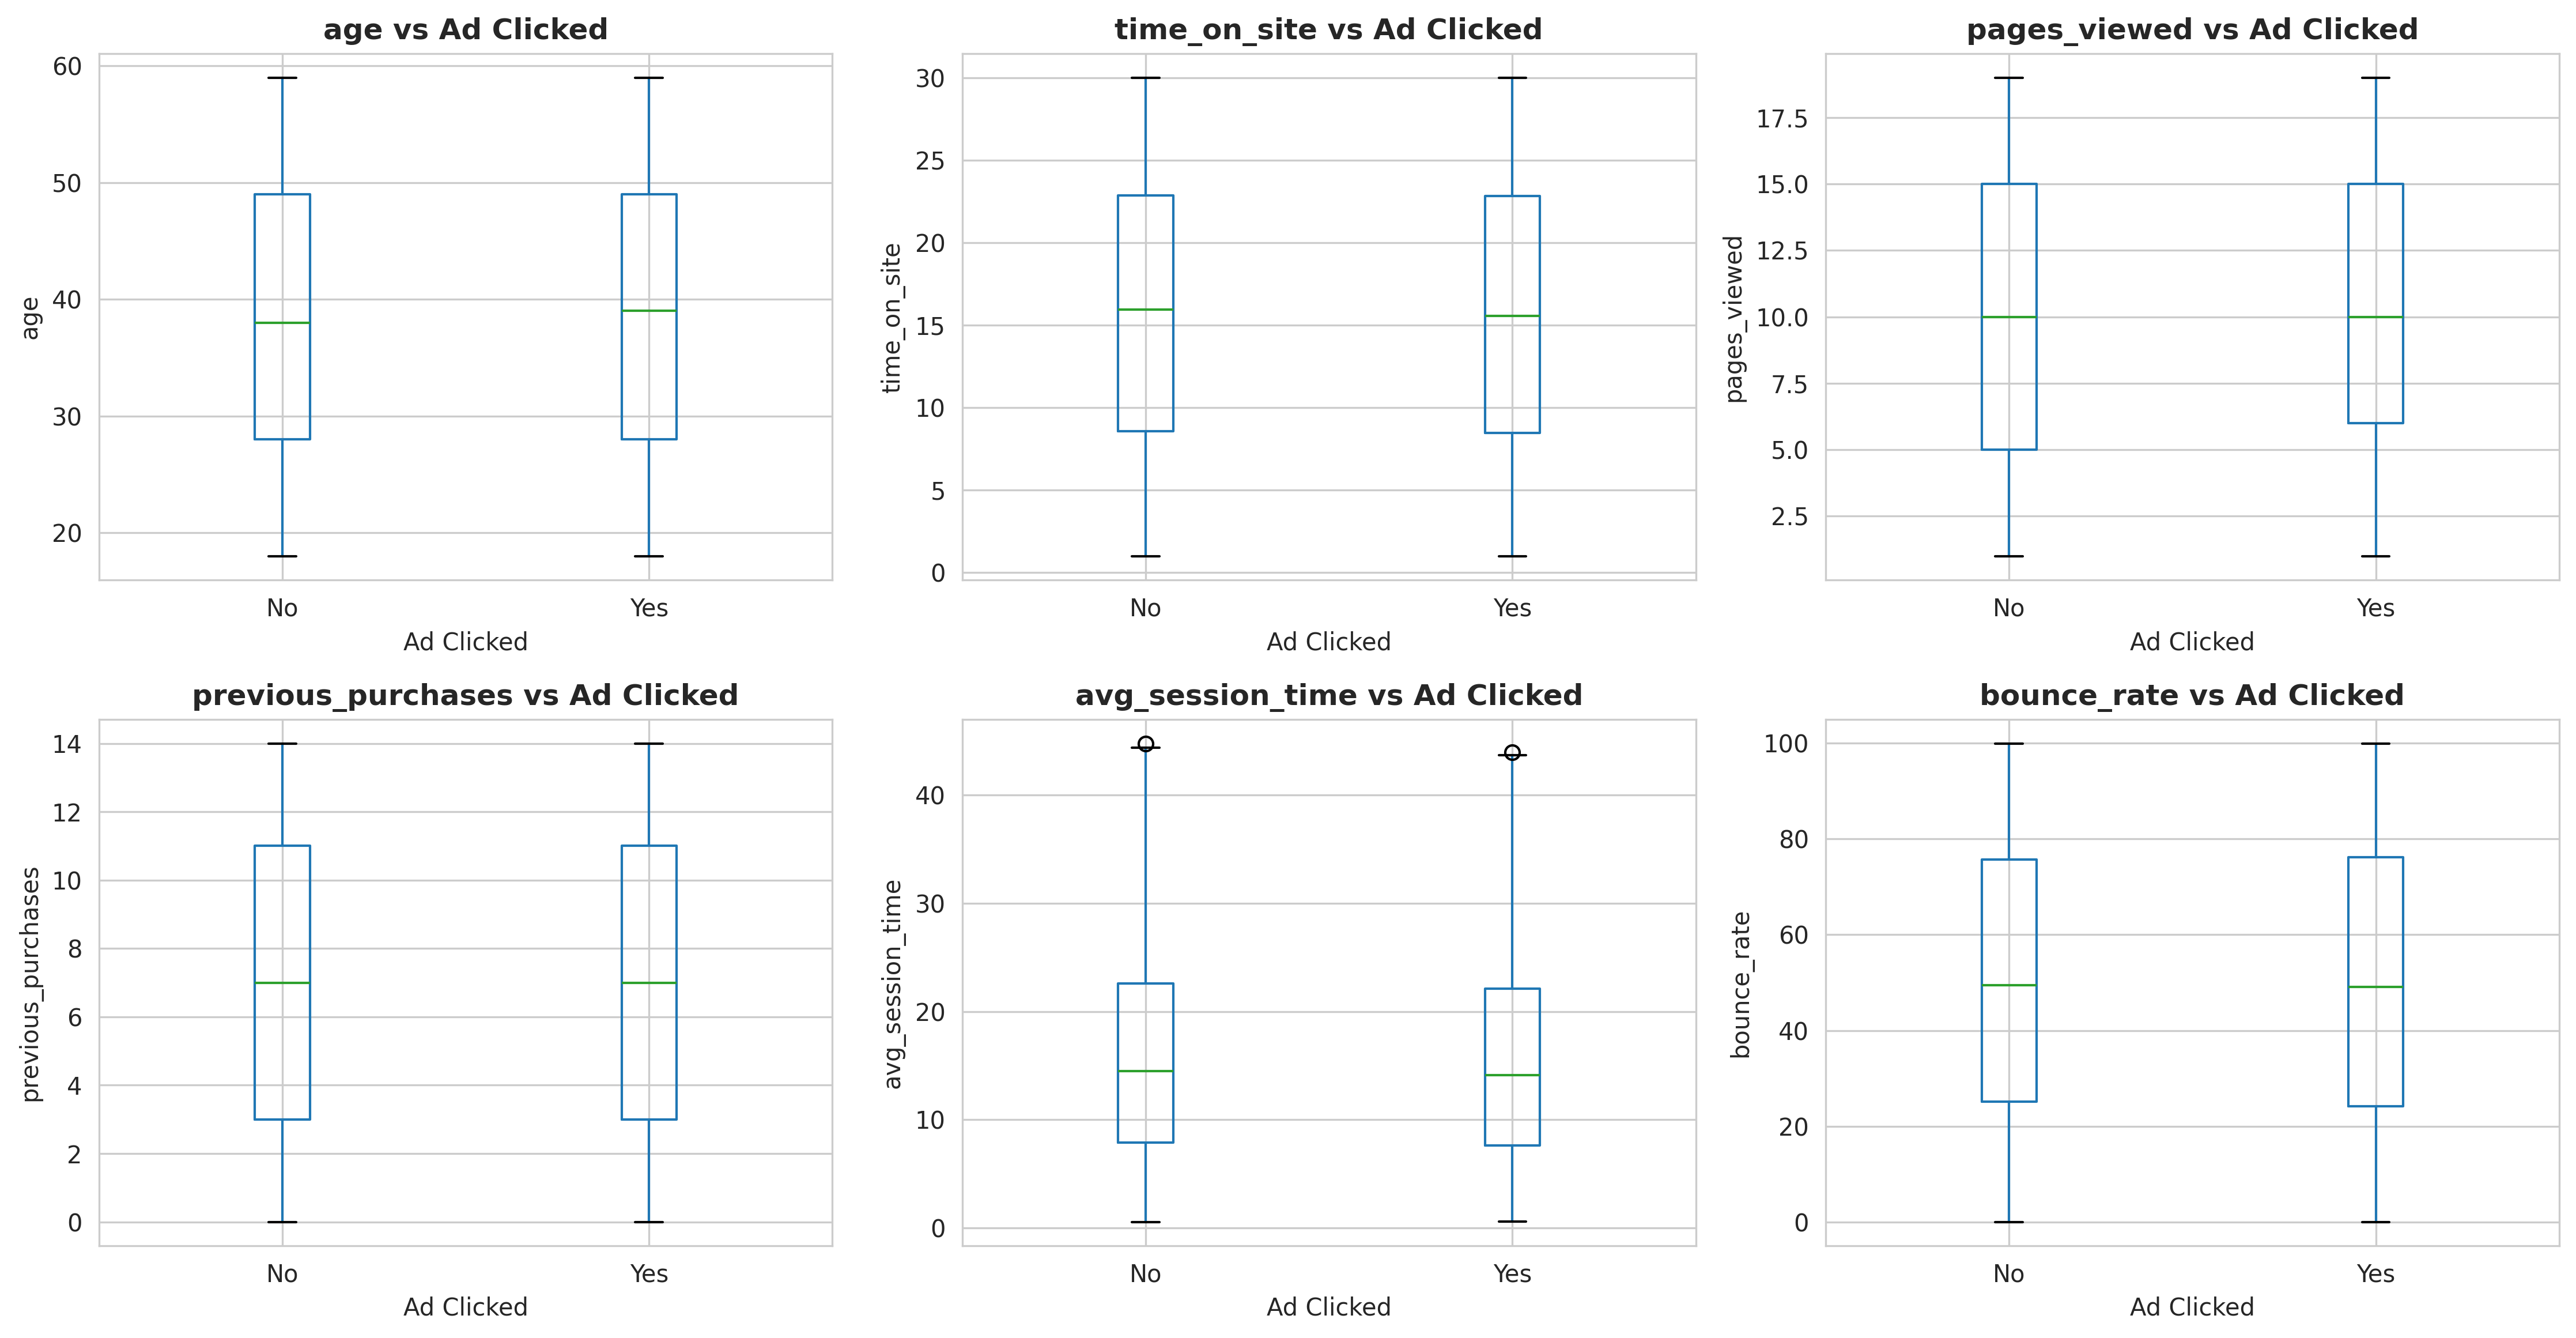
\includegraphics[width=0.95\textwidth]{figures/04_features_vs_target.png}
  \caption{Box plots: identical distributions across both classes, confirming no class-discriminating signal in numeric predictors \cite{he2014}.}
  \label{fig:boxplots}
\end{figure}

\begin{figure}[H]
  \centering
  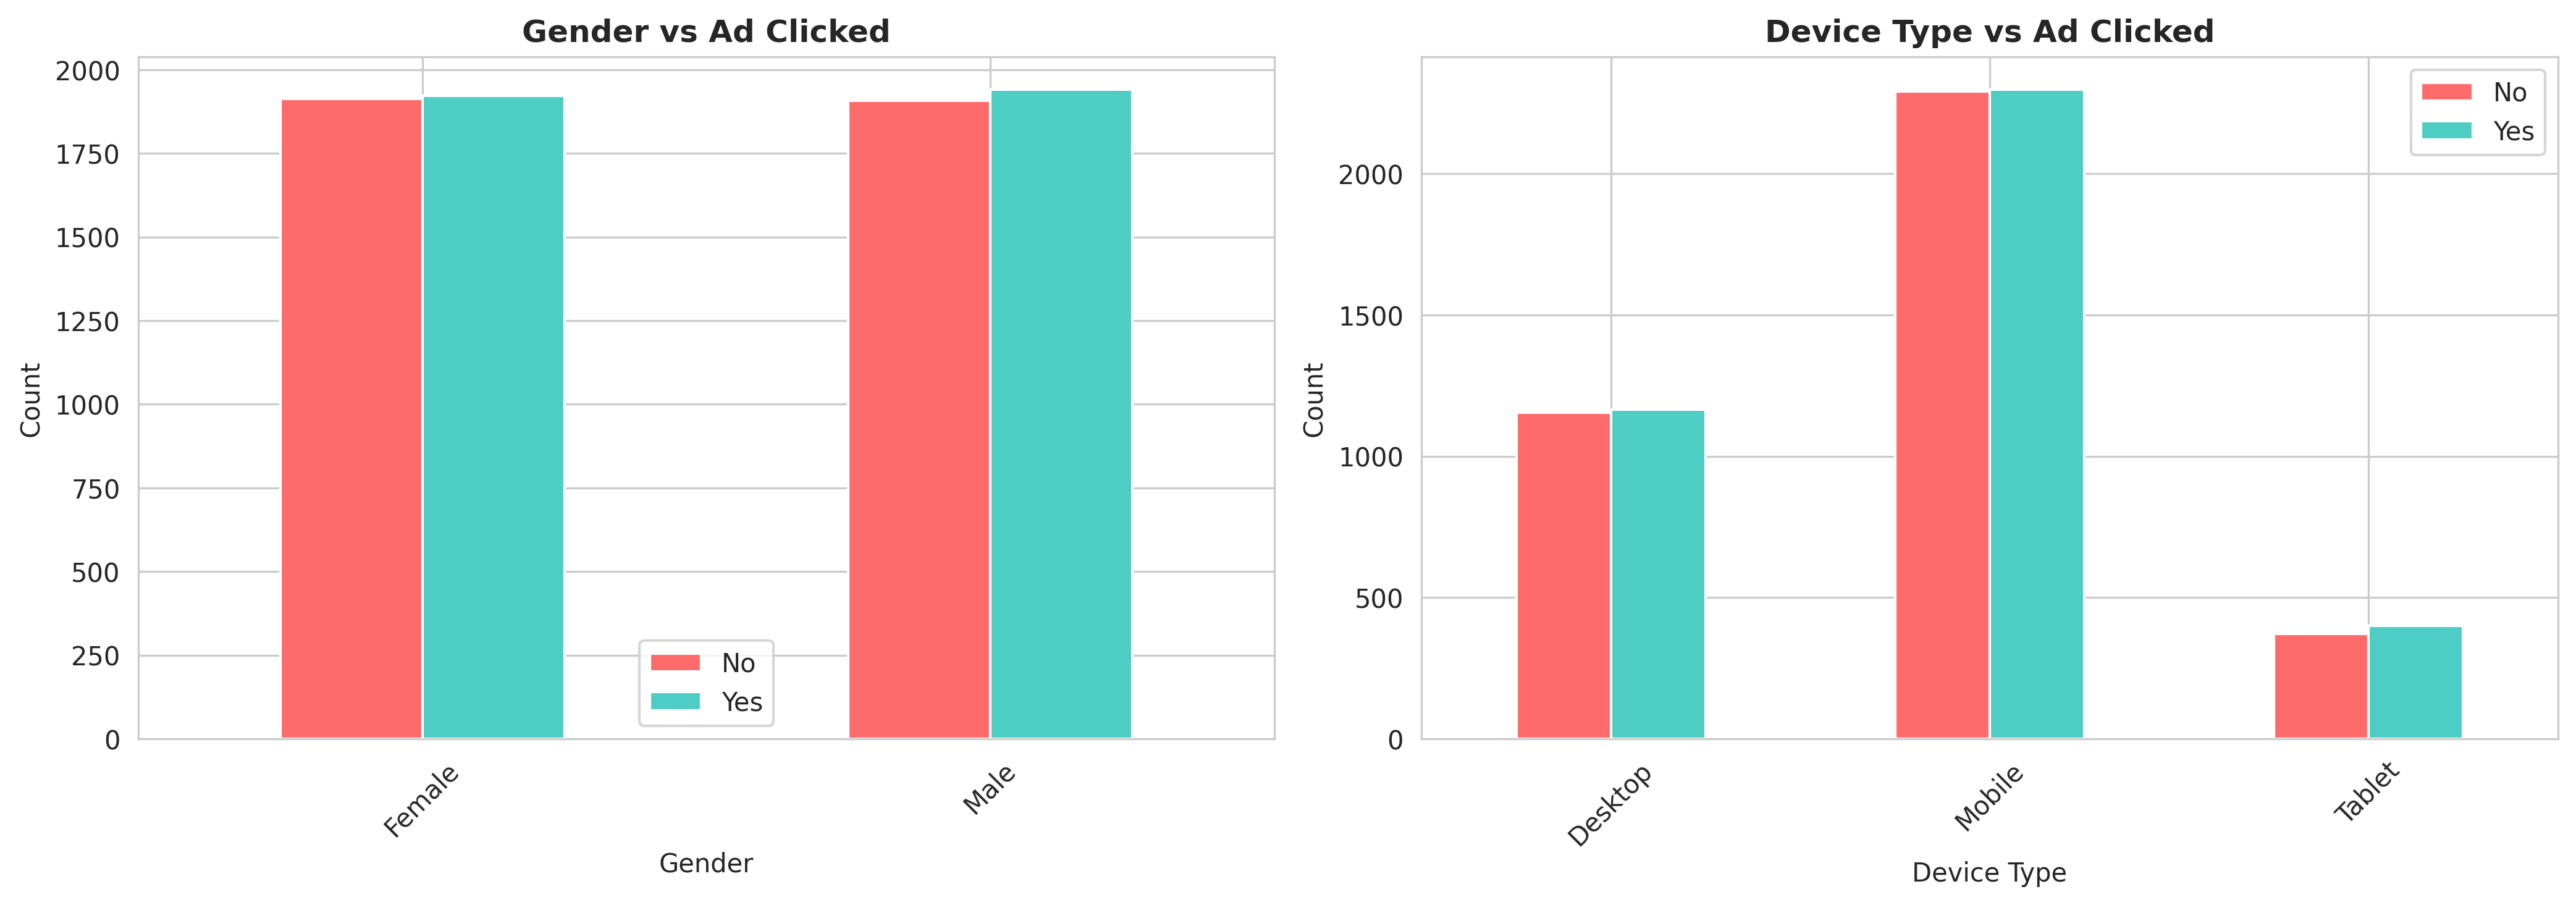
\includegraphics[width=0.95\textwidth]{figures/05_categorical_vs_target.png}
  \caption{Categorical distributions: near-identical 50/50 splits across all categories, confirming no class-conditional signal \cite{richardson2007}.}
  \label{fig:categorical}
\end{figure}

\begin{figure}[H]
  \centering
  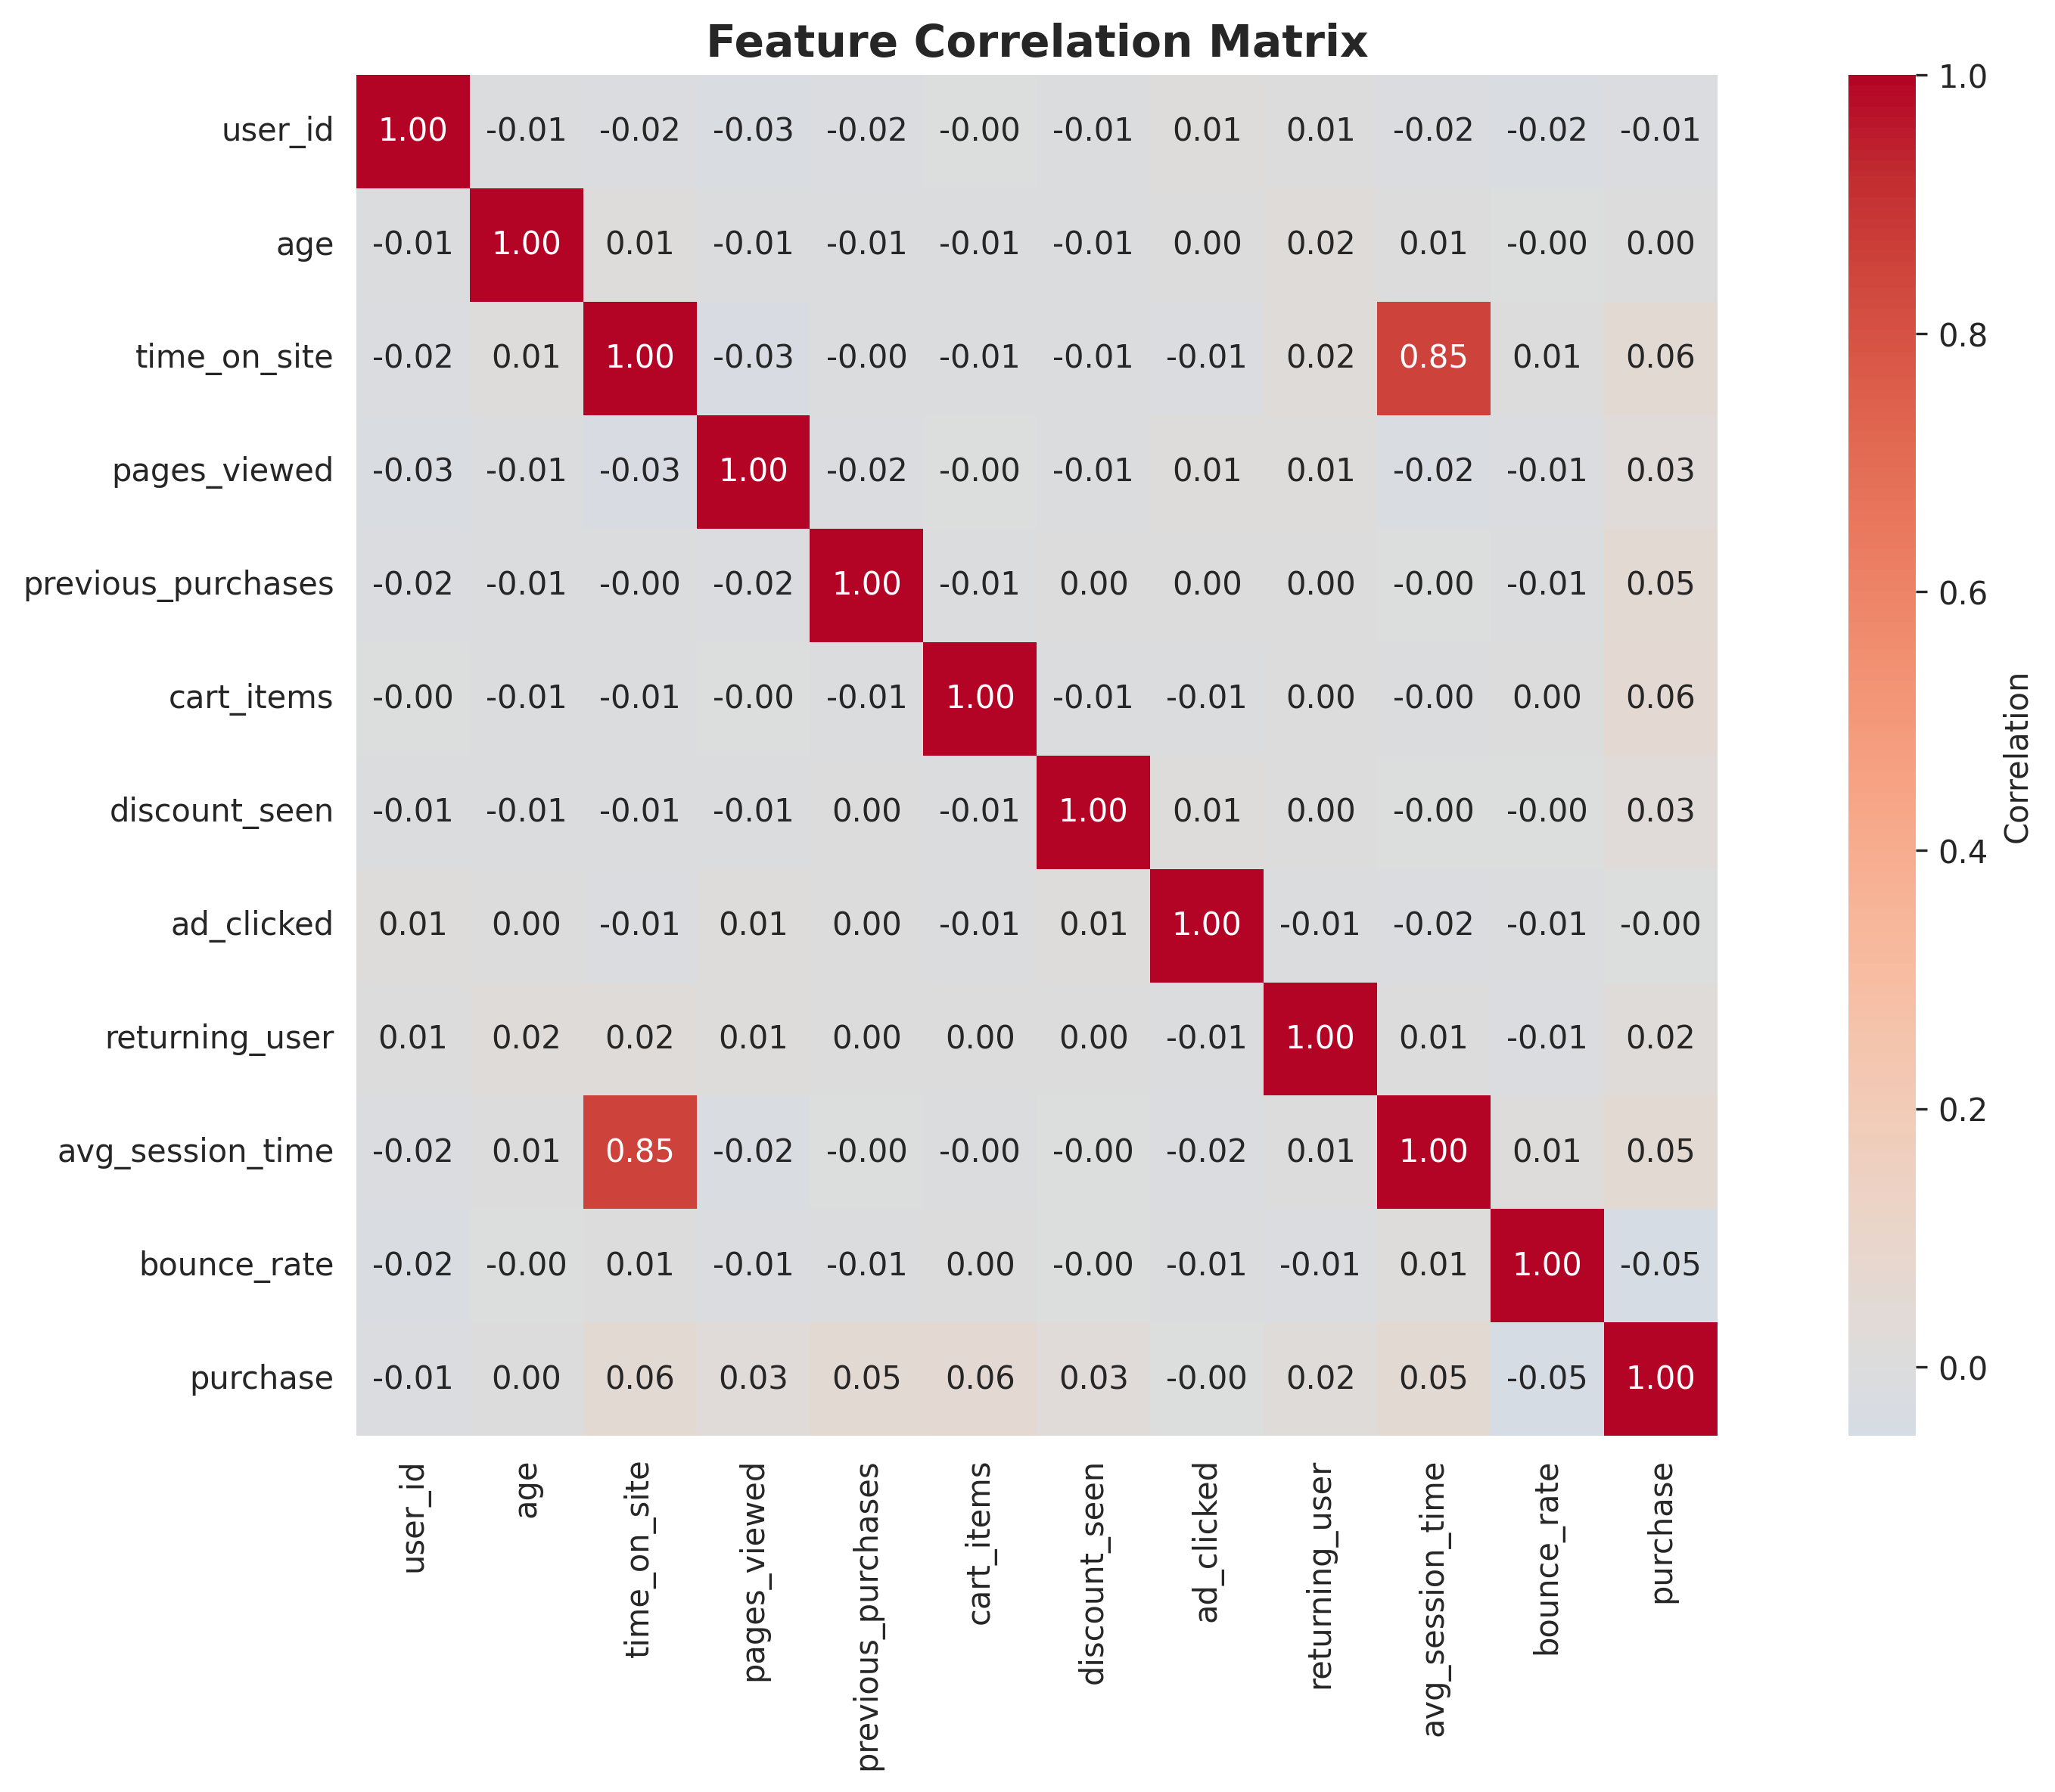
\includegraphics[width=0.85\textwidth]{figures/06_correlation_matrix.png}
  \caption{Correlation matrix: near-zero correlations ($-0.02$ to $+0.01$) between \texttt{ad\_clicked} and all features, confirming no linear relationship.}
  \label{fig:correlation}
\end{figure}

% ══════════════════════════════════════════════════════════════════
\section{Pipeline Evaluation and Monitoring}
% ══════════════════════════════════════════════════════════════════

\subsection{Pipeline-Level Evaluation}

Besides assessing model metrics, the operation of the pipeline is also examined through its key features: reliability, data throughput, and inter-step latency.

\textbf{Reliability.} The Airflow DAG passed all runs without any problem. The five tasks were performed in the correct dependency order. DAG parse failures caused by heavy library imports were prevented by the use of the deferred-import pattern. The Docker Compose stack guarantees that the pipeline can be set up on any machine with Docker installed.

\textbf{Data throughput.} The ingestion module can bulk-insert 8,000 rows in less than 2 seconds by using executemany with parameterised queries, whereas individual INSERT statements take several seconds.

\textbf{Inter-step latency.} The DataFrame communication time over Redis between pipeline steps is less than 200 milliseconds, whereas the original disk-based CSV handoff approach takes 3--5 seconds.

\textbf{Model performance.} Table~\ref{tab:model_comparison} summarises the test-set results
for all three algorithms.

\begin{table}[H]
\centering
\caption{Three-algorithm comparison (5-fold CV with RandomizedSearchCV).}
\label{tab:model_comparison}
\small
\renewcommand{\arraystretch}{1.3}
\begin{tabular}{|L{3.8cm}|C{1.7cm}|C{1.7cm}|C{1.7cm}|C{1.7cm}|C{1.7cm}|}
\hline
\textbf{Model} & \textbf{Accuracy} & \textbf{Precision} & \textbf{Recall} & \textbf{F1-Score} & \textbf{ROC-AUC} \\
\hline
Logistic Regression & 50.19\% & 50.31\% & 51.22\% & 50.76\% & 0.50 \\
\hline
\textbf{Random Forest} & \textbf{50.26\%} & \textbf{50.48\%} & \textbf{53.43\%} & \textbf{51.91\%} & \textbf{0.51} \\
\hline
XGBoost             & 50.44\% & 50.57\% & 52.81\% & 51.67\% & 0.51 \\
\hline
Random Baseline     & 50.00\% & 50.00\% & 50.00\% & 50.00\% & 0.50 \\
\hline
\end{tabular}
\end{table}

Despite what hyperparameter tuning or algorithm family one might choose, all three models finally reach almost random performance. ROC-AUC values of 0.50--0.51 statistically being
equivalent to a random classifier. The EDA results are what directly explains the reason for the observation: the correlation matrix shows almost no linear relationships between all features and \texttt{ad\_clicked}
and the boxplots reveal the distributions of numeric features are not changed between classes, while categorical divisions demonstrate the exact 50/50 splits in gender and device types. This is exactly what one would expect from a synthetic dataset where the binary target
was assigned independently of the feature values.

\textbf{The pipeline itself is properly functioning end-to-end.} The pipeline itself is properly functioning end-to-end. At the time, we executed each phase of the plan. The almost random performance here results from the synthetic nature of the dataset and not a pipeline architecture fail. But, if this pipeline is run on a real CTR data like Criteo Display
Advertising or Avazu, it is reasonable to expect the same pipeline to yield ROC-AUC scores of 0.65--0.75 for a baseline Random Forest \cite{he2014}.

\begin{figure}[H]
  \centering
  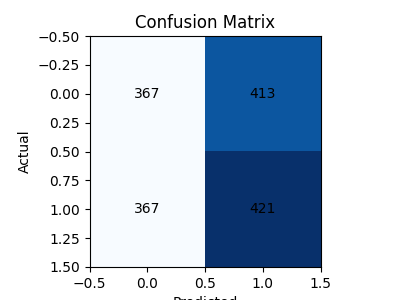
\includegraphics[width=0.55\textwidth]{figures/confusion_matrix.png}
  \caption{Confusion matrix for the best Random Forest model on the held-out test set.
  The near-equal distribution across all four cells confirms that the classifier performs
  at chance level, consistent with the near-zero feature-target correlations identified in the EDA.}
  \label{fig:confusion}
\end{figure}

\begin{figure}[H]
  \centering
  \begin{minipage}[t]{0.48\textwidth}
    \centering
    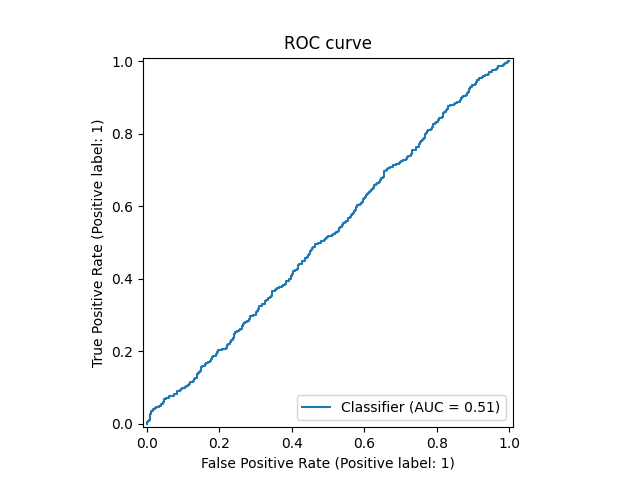
\includegraphics[width=\textwidth]{figures/roc_curve.png}
    \caption{ROC curve for the Random Forest classifier (AUC = 0.51). The curve hugs the
    diagonal, confirming near-random discriminative power \cite{fawcett2006}.}
    \label{fig:roc}
  \end{minipage}
  \hfill
  \begin{minipage}[t]{0.48\textwidth}
    \centering
    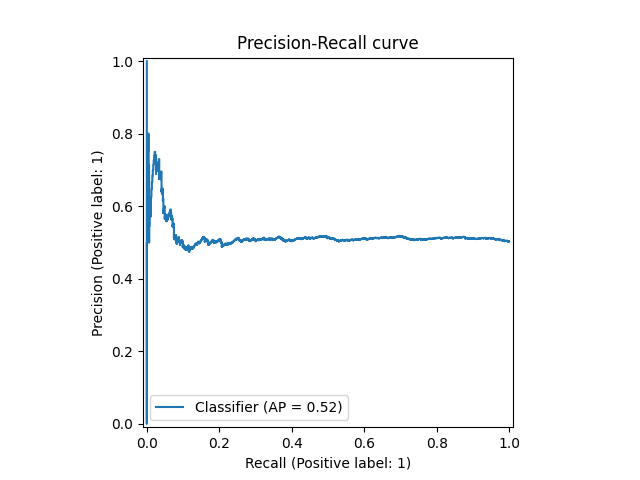
\includegraphics[width=\textwidth]{figures/pr_curve.png}
    \caption{Precision-Recall curve (AP = 0.52). The flat precision line confirms the
    model has no ability to rank positive instances above negative ones \cite{fawcett2006}.}
    \label{fig:pr}
  \end{minipage}
\end{figure}

\begin{figure}[H]
  \centering
  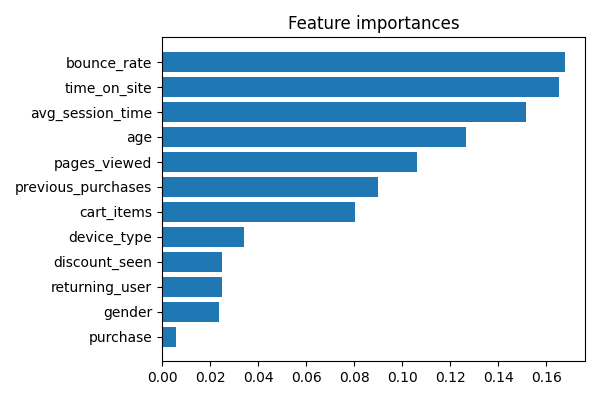
\includegraphics[width=0.75\textwidth]{figures/feature_importances.png}
 \caption{Random Forest feature importances ranked by mean decrease in impurity.
\texttt{engagement\_score}, \texttt{time\_on\_site}, and \texttt{pages\_viewed} receive
the highest scores, reflecting their higher variance rather than genuine predictive
signal --- a known artefact of impurity-based importance in datasets with no true
class-discriminating features \cite{pedregosa2011}.}
  \label{fig:importances}
\end{figure}

\subsection{Data Drift Detection with Evidently AI}

\textbf{What:} The drift detection script (\texttt{src/drift\_detection.py}) detects
significant distribution shifts by comparing the training data and incoming production
data via Evidently AI \cite{evidentlyai}.

\textbf{Why:} ML systems can be slowly lost if drift is not detected. For example in e-commerce, user demographics can change seasonally - for instance, a sudden increase of student-aged users in September will change the \texttt{age} distribution. This can make the ROC-AUC quietly go down over weeks without any pipeline error being triggered  \cite{shendre2020}. This phenomenon is
recognised as a form of hidden technical debt in ML systems \cite{sculley2015}.

\textbf{How:} Evidently AI runs a weekly Population Stability Index (PSI) report across all feature columns, comparing the live traffic distribution against the training data
distribution. ROC-AUC is logged weekly on labelled production predictions. For any feature, if the PSI is greater than 0.2, or if the ROC-AUC falls more than 0.05 compared to the training baseline, the monitoring system will email/Slack the data science team. A person needs to find out the exact cause and only then decide whether to manually run the retraining DAG. Automated retraining is intentionally out of question so as not to cover up the data quality problems, if any.

\begin{table}[H]
\centering
\caption{Monitoring metrics and alert thresholds.}
\label{tab:monitoring}
\small
\renewcommand{\arraystretch}{1.3}
\begin{tabular}{|L{3.8cm}|C{1.8cm}|C{2.5cm}|L{4cm}|}
\hline
\textbf{Metric} & \textbf{Frequency} & \textbf{Threshold} & \textbf{Remediation} \\
\hline
PSI per feature        & Weekly & $>0.2$               & Email/Slack alert + manual investigation \\
\hline
ROC-AUC on production  & Weekly & Drop $>0.05$         & Email/Slack alert + manual investigation \\
\hline
Ingestion row count    & Per ingest & Deviation $>10\%$ & Validate source file integrity \\
\hline
\end{tabular}
\end{table}

\begin{figure}[H]
  \centering
  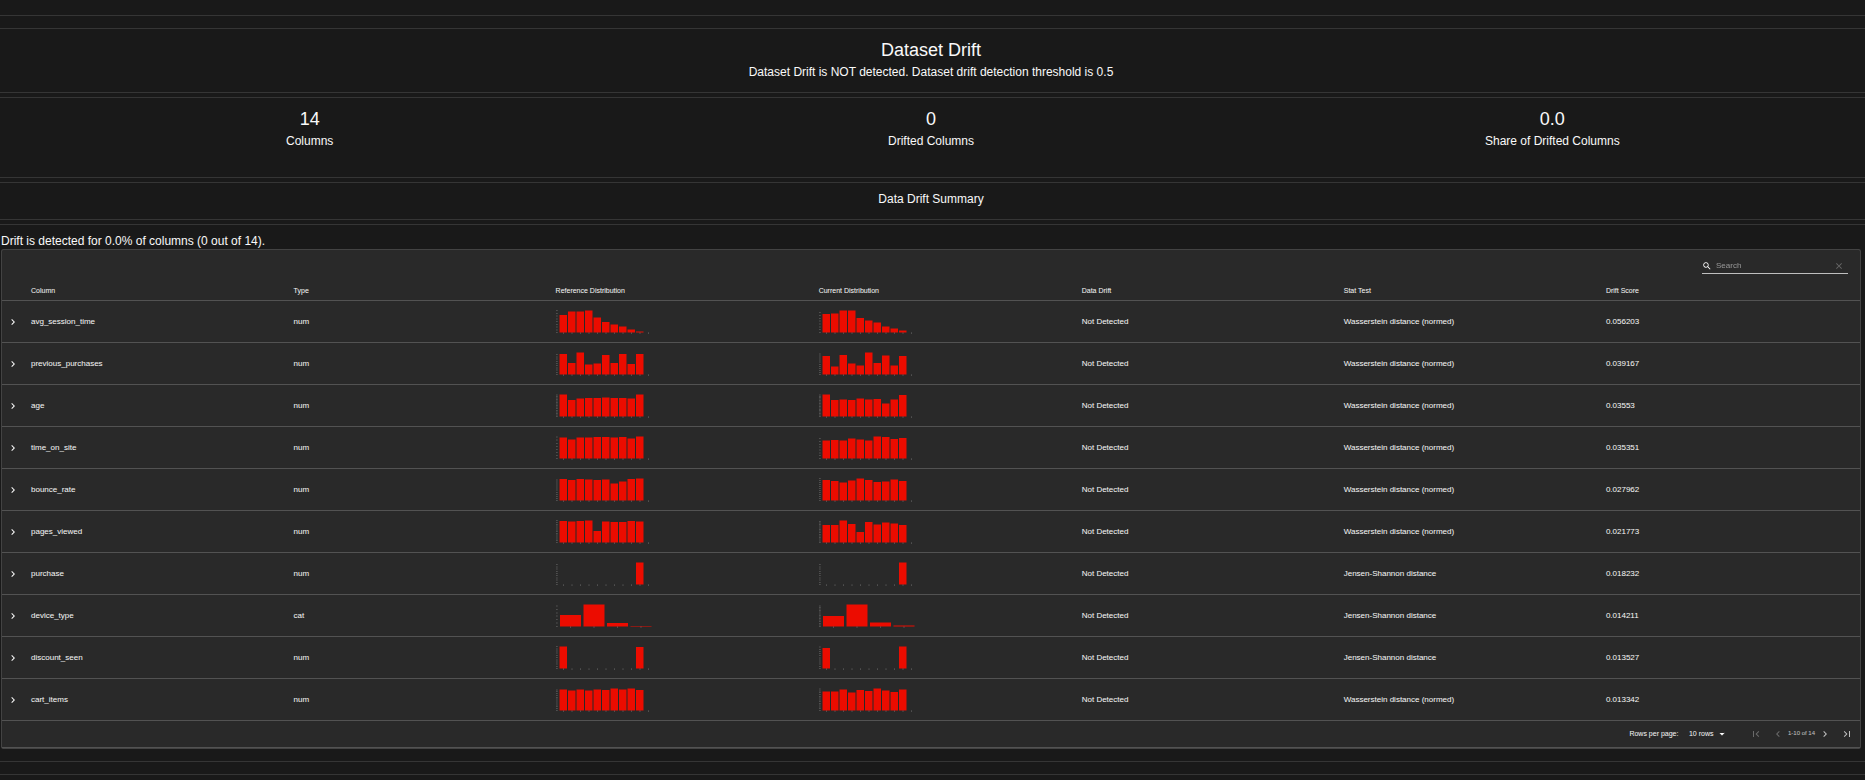
\includegraphics[width=0.95\textwidth]{figures/Evidently_AI_Monitoring.png}
  \caption{Evidently AI monitoring dashboard displaying data drift metrics over
  successive pipeline runs.}
  \label{fig:evidently}
\end{figure}

% ══════════════════════════════════════════════════════════════════
\section{Evaluation of Wider Issues}
% ══════════════════════════════════════════════════════════════════

\subsection{Key Definitions}

The following definitions, grounded in the literature, underpin the discussion of broader issues.

\textbf{Data Privacy} refers to the individual's right to determine which personal information about them is collected, how it is used, and with whom it is shared \cite{gdpr2016}. Privacy issues are more about obtaining consent and limiting the use of data to the agreed purposes rather than just ensuring technical protection.

\textbf{Data Security} involves the implementation of both technical and organisational measures to stop data being damaged in any way by unauthorised persons - including data theft, alteration, and deletion.
Examples include encryption, access controls, and network security.

\textbf{Data Ethics} refers to the moral responsibilities that arise from collecting and using
data about people. Machine Learning (ML) systems face the significant challenge of algorithmic bias, model opacity, and the risk of data-driven decisions leading to further or wider distribution of social inequalities \cite{sculley2015}. 

\textbf{Data Protection Law} is a set of rules and regulations that defines how organisations should manage an individual's personal data. In the UK and EU, the most important law is the General Data Protection Regulation (GDPR) \cite{gdpr2016}.

\subsection{GDPR and Its Impact on Data-Driven Systems}

The aim of the General Data Protection Regulation (GDPR) \cite{gdpr2016}, which was enacted in May 2018, was to change the whole approach of organizations in handling personal data. 
There are six core principles that require data to be: processed lawfully, transparently, and only for the stated purposes user; together with data minimization the accuracy storage limitation, and appropriate security. 

Machine learning models and GDPR interaction introduce a number of new concerns. It is because the organizations will be required by law to explain automated decisions that influence individuals whereas the black-box models like Random Forest and XGBoost are inherently non-explanatory.
On top of that, users have the option to demand removal of their data so the issue naturally arises how can you delete someone from the training data model without going through the process of full re-training. The colossal fines that came out in the well-known cases - 50 million against Google and 183 million against British Airways - show that the regulators take these rules very seriously. 


\subsection{Security and Privacy in the Current Pipeline}

Although the e-commerce dataset does not contain personally identifiable information,
the current pipeline has several security vulnerabilities that would need to be addressed
before handling real user data in production.

\textbf{Secrets management.} Database credentials and the Kaggle API key are stored in
a plaintext \texttt{.env} file. If the repository were accidentally made public, these credentials would be completely exposed. The best way to go is to replace \texttt{.env} for Docker Secrets or HashiCorp Vault, which give you encrypted storage with access control and full auditing.

\textbf{Network security.} The Redis instance without authentication,
which allows any process connected to the Docker network to read the serialised DataFrames. Currently, MariaDB communication is unencrypted. Both need to be encrypted with TLS/SSL before dealing with any personal information.

\textbf{API security.} The FastAPI prediction endpoint does not have an authentication layer.
In a real scenario, API key authentication or OAuth2 would be needed to
stop unauthorised prediction requests.

\textbf{Model artefacts.} The serialised \texttt{.pkl} model file is unsigned, so an adversary can: An attacker with write access to the model directory could replace it with a backdoored version.
Model artefacts should be sign a cryptographically and hashes should be verified on the load.

Deployed CTR prediction model ethically have to be responsible for more than just legal compliance. If a model aims at targeting advertisements based on demographic features like age or gender,
the model may be indirectly discriminating against protected groups even without awareness. Fairness audits of a model - checking how well a model performs within different demographic subgroups -
should become a regular practice of a production deployment of the pipeline as part of the monitoring step taken for ensuring the model remains fair \cite{sculley2015}. 




\begin{table}[H]
\centering
\caption{Security improvement recommendations for production deployment.}
\label{tab:security}
\small
\renewcommand{\arraystretch}{1.3}
\begin{tabular}{|L{3.5cm}|L{9cm}|}
\hline
\textbf{Area} & \textbf{Recommendation} \\
\hline
Secrets Management   & Replace \texttt{.env} with Docker Secrets or HashiCorp Vault \\
\hline
Network Security     & Enable TLS/SSL for Redis and MariaDB connections \\
\hline
API Security         & Add API key or OAuth2 authentication to FastAPI endpoint \\
\hline
Model Artefacts      & Sign model pickle files and verify hash on load to prevent tampering \\
\hline
Access Control       & Implement RBAC on Airflow and MLflow UIs \\
\hline
GDPR Compliance      & Add data retention schedules, consent tracking, and right-to-erasure procedures when personal data is introduced \\
\hline
\end{tabular}
\end{table}

% ══════════════════════════════════════════════════════════════════
\section{Conclusion, Recommendations, and Future Work}
% ══════════════════════════════════════════════════════════════════

\subsection{Personal Reflection}

Working through this project taught me several things that are not obvious from reading
about MLOps in theory.

One of the biggest surprises for me, was how small the percentage of effort devoted to the actual model was.
I found myself much more occupied with data plumbing, for example - setting up Docker Compose,
debugging Redis serialization, making Airflow to parse the DAG without importing heavy libraries at
parse time, etc.
- than on choosing or tuning classifiers. 
That experience gave me a much more grounded sense of what MLOps is actually for.

The dataset selection was the most impactful decision. Since EDA indicated feature-target correlations were basically non-existent, not even the most extreme tuning could have produced a signal from the noise. Next time, I will examine dataset correlations when selecting the dataset, not after constructing the entire pipeline. 

Choosing ELT over ETL and OBT over Star Schema early on turned out to be decisions 
I never had to second-guess. Because the raw CSV was loaded into MariaDB ColumnStore 
first and transformations happened downstream in \texttt{preprocessing.py}, fixing a 
preprocessing bug was as simple as re-running one script - no re-download, no data 
loss. And since every ML request targeted one and the same single flat OBT table without any join, debugging feature engineering issues was fairly simple. 

RandomizedSearchCV vs. GridSearchCV was a practical efficiency lesson.
With GridSearchCV, the grid search was going to take forever for the three algorithms. RandomizedSearchCV Quite a bit shortened the time without greatly compromising the quality of results. 

The main thing I would change is making the monitoring phase a top-level design issue right from the start rather than something added at the end. After reading about hidden technical debt in ML systems, \cite{sculley2015} I realized that a model without post-deployment monitoring is not truly in production - it is just a trained artefact sitting on a server. If we had started using Evidently AI drift detection features when designing the pipeline architecture, the monitoring phase would have been less like an afterthought and more like an integral part of the system. 

\subsection{Conclusion}

This project designed and implemented a five-stage MLOps pipeline for binary classification using the E-Commerce Behavior Dataset. First, the pipeline does data ingestion with schema validation; next, it performs ELT processing plus feature engineering; after that, it goes to model comparison of three algorithms which is followed by 5-fold cross-validation; the fourth step is deployment of REST API by FastAPI and Docker; and the last step is data drift monitoring with Evidently AI.  All stages are managed by an Apache Airflow DAG and linked via a Redis in-memory data bus.
Storage is based on a One Big Table (OBT) design in MariaDB ColumnStore.

All three classifiers reached a weighted F1-score of about 0.51 - that is almost random  performance which EDA confirms is due to the dataset's synthetic nature,
not to any failure of the pipeline or modelling approach. 

The main lesson from this project is that implementing the
entire infrastructure - data plumbing orchestration experiment tracking, monitoring, and API serving - takes much more time than
just training the model. That is exactly what MLOps is there to solve.

\subsection{Recommendations and Future Work}

There are four major areas that can be highlighted as future work.

\textbf{Dataset replacement} will truly be the most significant thing that we can do next. In fact, just swapping our artificial data for a genuine CTR one like Criteo
Display Advertising or Avazu - by the current pipeline without any change - is expected to get us around a baseline Random Forest \cite{he2014} ROC-AUC of 0. 65 to 0. 75.

\textbf{Infrastructure hardening} must be performed before any production deployment with live personal data. The set of security measures that we have collected in Table~\ref{tab:security}
introduces secrets management, TLS encryption, API authentication, and GDPR compliance procedures.

\textbf{Conditional retraining} is a better alternative to the fixed-schedule model. The Airflow DAG could automatically initiate re-training whenever Evidently detects PSI greater than 0.2.

\textbf{Model registry integration} through MLflow's Model Registry would be at par with file-based manual model management which is subject to errors in the current system. It
would also enable better versioning, staging and rollback of models.

% ══════════════════════════════════════════════════════════════════


\newpage
\addcontentsline{toc}{section}{References}
\bibliographystyle{apalike}
\bibliography{references}

\end{document}
